\documentclass[twoside]{book}

% Packages required by doxygen
\usepackage{fixltx2e}
\usepackage{calc}
\usepackage{doxygen}
\usepackage[export]{adjustbox} % also loads graphicx
\usepackage{graphicx}
\usepackage[utf8]{inputenc}
\usepackage{makeidx}
\usepackage{multicol}
\usepackage{multirow}
\PassOptionsToPackage{warn}{textcomp}
\usepackage{textcomp}
\usepackage[nointegrals]{wasysym}
\usepackage[table]{xcolor}

% Font selection
\usepackage[T1]{fontenc}
\usepackage[scaled=.90]{helvet}
\usepackage{courier}
\usepackage{amssymb}
\usepackage{sectsty}
\renewcommand{\familydefault}{\sfdefault}
\allsectionsfont{%
  \fontseries{bc}\selectfont%
  \color{darkgray}%
}
\renewcommand{\DoxyLabelFont}{%
  \fontseries{bc}\selectfont%
  \color{darkgray}%
}
\newcommand{\+}{\discretionary{\mbox{\scriptsize$\hookleftarrow$}}{}{}}

% Page & text layout
\usepackage{geometry}
\geometry{%
  a4paper,%
  top=2.5cm,%
  bottom=2.5cm,%
  left=2.5cm,%
  right=2.5cm%
}
\tolerance=750
\hfuzz=15pt
\hbadness=750
\setlength{\emergencystretch}{15pt}
\setlength{\parindent}{0cm}
\setlength{\parskip}{3ex plus 2ex minus 2ex}
\makeatletter
\renewcommand{\paragraph}{%
  \@startsection{paragraph}{4}{0ex}{-1.0ex}{1.0ex}{%
    \normalfont\normalsize\bfseries\SS@parafont%
  }%
}
\renewcommand{\subparagraph}{%
  \@startsection{subparagraph}{5}{0ex}{-1.0ex}{1.0ex}{%
    \normalfont\normalsize\bfseries\SS@subparafont%
  }%
}
\makeatother

% Headers & footers
\usepackage{fancyhdr}
\pagestyle{fancyplain}
\fancyhead[LE]{\fancyplain{}{\bfseries\thepage}}
\fancyhead[CE]{\fancyplain{}{}}
\fancyhead[RE]{\fancyplain{}{\bfseries\leftmark}}
\fancyhead[LO]{\fancyplain{}{\bfseries\rightmark}}
\fancyhead[CO]{\fancyplain{}{}}
\fancyhead[RO]{\fancyplain{}{\bfseries\thepage}}
\fancyfoot[LE]{\fancyplain{}{}}
\fancyfoot[CE]{\fancyplain{}{}}
\fancyfoot[RE]{\fancyplain{}{\bfseries\scriptsize Generated by Doxygen }}
\fancyfoot[LO]{\fancyplain{}{\bfseries\scriptsize Generated by Doxygen }}
\fancyfoot[CO]{\fancyplain{}{}}
\fancyfoot[RO]{\fancyplain{}{}}
\renewcommand{\footrulewidth}{0.4pt}
\renewcommand{\chaptermark}[1]{%
  \markboth{#1}{}%
}
\renewcommand{\sectionmark}[1]{%
  \markright{\thesection\ #1}%
}

% Indices & bibliography
\usepackage{natbib}
\usepackage[titles]{tocloft}
\setcounter{tocdepth}{3}
\setcounter{secnumdepth}{5}
\makeindex

% Hyperlinks (required, but should be loaded last)
\usepackage{ifpdf}
\ifpdf
  \usepackage[pdftex,pagebackref=true]{hyperref}
\else
  \usepackage[ps2pdf,pagebackref=true]{hyperref}
\fi
\hypersetup{%
  colorlinks=true,%
  linkcolor=blue,%
  citecolor=blue,%
  unicode%
}

% Custom commands
\newcommand{\clearemptydoublepage}{%
  \newpage{\pagestyle{empty}\cleardoublepage}%
}

\usepackage{caption}
\captionsetup{labelsep=space,justification=centering,font={bf},singlelinecheck=off,skip=4pt,position=top}

%===== C O N T E N T S =====

\begin{document}

% Titlepage & ToC
\hypersetup{pageanchor=false,
             bookmarksnumbered=true,
             pdfencoding=unicode
            }
\pagenumbering{roman}
\begin{titlepage}
\vspace*{7cm}
\begin{center}%
{\Large Reht\+Se }\\
\vspace*{1cm}
{\large Generated by Doxygen 1.8.11}\\
\end{center}
\end{titlepage}
\clearemptydoublepage
\tableofcontents
\clearemptydoublepage
\pagenumbering{arabic}
\hypersetup{pageanchor=true}

%--- Begin generated contents ---
\chapter{Rehtse}
\label{md__home_xshell_git_RehtSe_README}
\hypertarget{md__home_xshell_git_RehtSe_README}{}
br\+\_\+netfilter+\+Iptables+\+N\+F\+Queue+\+B\+P\+F+\+Regex ---$>$ Easy way to modify network packets on the fly!

Thanks to\+:

\href{https://github.com/pellegre/libcrafter}{\tt https\+://github.\+com/pellegre/libcrafter} \href{https://github.com/ytakano/radix_tree}{\tt https\+://github.\+com/ytakano/radix\+\_\+tree}

Both of them maid things to work here.

You will need\+: \begin{DoxyVerb}apt-get install libboost-all-dev libnetfilter-queue1 libnetfilter-queue-dev libpcap0.8 libpcap0.8-dev
Follow instructions to install libcrafter. 
\end{DoxyVerb}


To use it\+: \begin{DoxyVerb}1 cd Debug; make clean; make all;
2 edit your config.json file. Take a look at Debug/config.json for an example.
3 write your iptables rule to dispatch packets to Rehtse -> iptables -A FORWARD -j NFQUEUE --queue-num 0.
4 just ./RehtSe
\end{DoxyVerb}


The project works now on Eclipse Neon. 
\chapter{Hierarchical Index}
\section{Class Hierarchy}
This inheritance list is sorted roughly, but not completely, alphabetically\+:\begin{DoxyCompactList}
\item \contentsline{section}{Flow}{\pageref{class_flow}}{}
\begin{DoxyCompactList}
\item \contentsline{section}{Generic\+Flow}{\pageref{class_generic_flow}}{}
\item \contentsline{section}{T\+C\+P\+Flow}{\pageref{class_t_c_p_flow}}{}
\end{DoxyCompactList}
\item \contentsline{section}{Flow\+Tracker}{\pageref{class_flow_tracker}}{}
\item iterator\begin{DoxyCompactList}
\item \contentsline{section}{radix\+\_\+tree\+\_\+it$<$ K, T $>$}{\pageref{classradix__tree__it}}{}
\end{DoxyCompactList}
\item \contentsline{section}{nfq\+\_\+data}{\pageref{structnfq__data}}{}
\item \contentsline{section}{N\+F\+Queue}{\pageref{class_n_f_queue}}{}
\item \contentsline{section}{Pattern}{\pageref{class_pattern}}{}
\item \contentsline{section}{radix\+\_\+tree$<$ K, T $>$}{\pageref{classradix__tree}}{}
\item \contentsline{section}{radix\+\_\+tree$<$ std\+:\+:string, Flow $\ast$ $>$}{\pageref{classradix__tree}}{}
\item \contentsline{section}{radix\+\_\+tree\+\_\+node$<$ K, T $>$}{\pageref{classradix__tree__node}}{}
\item \contentsline{section}{radix\+\_\+tree\+\_\+node$<$ std\+:\+:string, Flow $\ast$ $>$}{\pageref{classradix__tree__node}}{}
\item \contentsline{section}{Scanner}{\pageref{class_scanner}}{}
\item \contentsline{section}{User\+Interface}{\pageref{class_user_interface}}{}
\end{DoxyCompactList}

\chapter{Class Index}
\section{Class List}
Here are the classes, structs, unions and interfaces with brief descriptions\+:\begin{DoxyCompactList}
\item\contentsline{section}{\hyperlink{class_flow}{Flow} }{\pageref{class_flow}}{}
\item\contentsline{section}{\hyperlink{class_flow_tracker}{Flow\+Tracker} }{\pageref{class_flow_tracker}}{}
\item\contentsline{section}{\hyperlink{class_generic_flow}{Generic\+Flow} }{\pageref{class_generic_flow}}{}
\item\contentsline{section}{\hyperlink{structnfq__data}{nfq\+\_\+data} }{\pageref{structnfq__data}}{}
\item\contentsline{section}{\hyperlink{class_n_f_queue}{N\+F\+Queue} }{\pageref{class_n_f_queue}}{}
\item\contentsline{section}{\hyperlink{class_pattern}{Pattern} }{\pageref{class_pattern}}{}
\item\contentsline{section}{\hyperlink{classradix__tree}{radix\+\_\+tree$<$ K, T $>$} }{\pageref{classradix__tree}}{}
\item\contentsline{section}{\hyperlink{classradix__tree__it}{radix\+\_\+tree\+\_\+it$<$ K, T $>$} }{\pageref{classradix__tree__it}}{}
\item\contentsline{section}{\hyperlink{classradix__tree__node}{radix\+\_\+tree\+\_\+node$<$ K, T $>$} }{\pageref{classradix__tree__node}}{}
\item\contentsline{section}{\hyperlink{class_scanner}{Scanner} }{\pageref{class_scanner}}{}
\item\contentsline{section}{\hyperlink{class_t_c_p_flow}{T\+C\+P\+Flow} }{\pageref{class_t_c_p_flow}}{}
\item\contentsline{section}{\hyperlink{class_user_interface}{User\+Interface} }{\pageref{class_user_interface}}{}
\end{DoxyCompactList}

\chapter{File Index}
\section{File List}
Here is a list of all files with brief descriptions\+:\begin{DoxyCompactList}
\item\contentsline{section}{/home/xshell/git/\+Reht\+Se/\+Debug/src/\hyperlink{main_8d}{main.\+d} }{\pageref{main_8d}}{}
\item\contentsline{section}{/home/xshell/git/\+Reht\+Se/\+Debug/src/\hyperlink{misc_8d}{misc.\+d} }{\pageref{misc_8d}}{}
\item\contentsline{section}{/home/xshell/git/\+Reht\+Se/\+Debug/src/\hyperlink{_n_f_queue_8d}{N\+F\+Queue.\+d} }{\pageref{_n_f_queue_8d}}{}
\item\contentsline{section}{/home/xshell/git/\+Reht\+Se/\+Debug/src/\hyperlink{_u_i_8d}{U\+I.\+d} }{\pageref{_u_i_8d}}{}
\item\contentsline{section}{/home/xshell/git/\+Reht\+Se/\+Debug/src/\hyperlink{_user_interface_8d}{User\+Interface.\+d} }{\pageref{_user_interface_8d}}{}
\item\contentsline{section}{/home/xshell/git/\+Reht\+Se/\+Debug/src/flows/\hyperlink{_flow_8d}{Flow.\+d} }{\pageref{_flow_8d}}{}
\item\contentsline{section}{/home/xshell/git/\+Reht\+Se/\+Debug/src/flows/\hyperlink{_flow_tracker_8d}{Flow\+Tracker.\+d} }{\pageref{_flow_tracker_8d}}{}
\item\contentsline{section}{/home/xshell/git/\+Reht\+Se/\+Debug/src/flows/\hyperlink{_generic_flow_8d}{Generic\+Flow.\+d} }{\pageref{_generic_flow_8d}}{}
\item\contentsline{section}{/home/xshell/git/\+Reht\+Se/\+Debug/src/flows/\hyperlink{_peer_8d}{Peer.\+d} }{\pageref{_peer_8d}}{}
\item\contentsline{section}{/home/xshell/git/\+Reht\+Se/\+Debug/src/flows/\hyperlink{_t_c_p_flow_8d}{T\+C\+P\+Flow.\+d} }{\pageref{_t_c_p_flow_8d}}{}
\item\contentsline{section}{/home/xshell/git/\+Reht\+Se/\+Debug/src/pattern/\hyperlink{_pattern_8d}{Pattern.\+d} }{\pageref{_pattern_8d}}{}
\item\contentsline{section}{/home/xshell/git/\+Reht\+Se/\+Debug/src/pattern/\hyperlink{_scanner_8d}{Scanner.\+d} }{\pageref{_scanner_8d}}{}
\item\contentsline{section}{/home/xshell/git/\+Reht\+Se/include/\hyperlink{err_8h}{err.\+h} }{\pageref{err_8h}}{}
\item\contentsline{section}{/home/xshell/git/\+Reht\+Se/include/\hyperlink{misc_8h}{misc.\+h} }{\pageref{misc_8h}}{}
\item\contentsline{section}{/home/xshell/git/\+Reht\+Se/include/\hyperlink{_n_f_queue_8h}{N\+F\+Queue.\+h} }{\pageref{_n_f_queue_8h}}{}
\item\contentsline{section}{/home/xshell/git/\+Reht\+Se/include/\hyperlink{radix__tree_8hpp}{radix\+\_\+tree.\+hpp} }{\pageref{radix__tree_8hpp}}{}
\item\contentsline{section}{/home/xshell/git/\+Reht\+Se/include/\hyperlink{radix__tree__it_8hpp}{radix\+\_\+tree\+\_\+it.\+hpp} }{\pageref{radix__tree__it_8hpp}}{}
\item\contentsline{section}{/home/xshell/git/\+Reht\+Se/include/\hyperlink{radix__tree__node_8hpp}{radix\+\_\+tree\+\_\+node.\+hpp} }{\pageref{radix__tree__node_8hpp}}{}
\item\contentsline{section}{/home/xshell/git/\+Reht\+Se/include/\hyperlink{_user_interface_8h}{User\+Interface.\+h} }{\pageref{_user_interface_8h}}{}
\item\contentsline{section}{/home/xshell/git/\+Reht\+Se/include/flows/\hyperlink{_flow_8h}{Flow.\+h} }{\pageref{_flow_8h}}{}
\item\contentsline{section}{/home/xshell/git/\+Reht\+Se/include/flows/\hyperlink{_flow_tracker_8h}{Flow\+Tracker.\+h} }{\pageref{_flow_tracker_8h}}{}
\item\contentsline{section}{/home/xshell/git/\+Reht\+Se/include/flows/\hyperlink{_generic_flow_8h}{Generic\+Flow.\+h} }{\pageref{_generic_flow_8h}}{}
\item\contentsline{section}{/home/xshell/git/\+Reht\+Se/include/flows/\hyperlink{_t_c_p_flow_8h}{T\+C\+P\+Flow.\+h} }{\pageref{_t_c_p_flow_8h}}{}
\item\contentsline{section}{/home/xshell/git/\+Reht\+Se/include/pattern/\hyperlink{_pattern_8h}{Pattern.\+h} }{\pageref{_pattern_8h}}{}
\item\contentsline{section}{/home/xshell/git/\+Reht\+Se/include/pattern/\hyperlink{_scanner_8h}{Scanner.\+h} }{\pageref{_scanner_8h}}{}
\item\contentsline{section}{/home/xshell/git/\+Reht\+Se/src/\hyperlink{main_8cpp}{main.\+cpp} }{\pageref{main_8cpp}}{}
\item\contentsline{section}{/home/xshell/git/\+Reht\+Se/src/\hyperlink{misc_8cpp}{misc.\+cpp} }{\pageref{misc_8cpp}}{}
\item\contentsline{section}{/home/xshell/git/\+Reht\+Se/src/\hyperlink{_n_f_queue_8cpp}{N\+F\+Queue.\+cpp} }{\pageref{_n_f_queue_8cpp}}{}
\item\contentsline{section}{/home/xshell/git/\+Reht\+Se/src/\hyperlink{_user_interface_8cpp}{User\+Interface.\+cpp} }{\pageref{_user_interface_8cpp}}{}
\item\contentsline{section}{/home/xshell/git/\+Reht\+Se/src/flows/\hyperlink{_flow_8cpp}{Flow.\+cpp} }{\pageref{_flow_8cpp}}{}
\item\contentsline{section}{/home/xshell/git/\+Reht\+Se/src/flows/\hyperlink{_flow_tracker_8cpp}{Flow\+Tracker.\+cpp} }{\pageref{_flow_tracker_8cpp}}{}
\item\contentsline{section}{/home/xshell/git/\+Reht\+Se/src/flows/\hyperlink{_generic_flow_8cpp}{Generic\+Flow.\+cpp} }{\pageref{_generic_flow_8cpp}}{}
\item\contentsline{section}{/home/xshell/git/\+Reht\+Se/src/flows/\hyperlink{_t_c_p_flow_8cpp}{T\+C\+P\+Flow.\+cpp} }{\pageref{_t_c_p_flow_8cpp}}{}
\item\contentsline{section}{/home/xshell/git/\+Reht\+Se/src/pattern/\hyperlink{_pattern_8cpp}{Pattern.\+cpp} }{\pageref{_pattern_8cpp}}{}
\item\contentsline{section}{/home/xshell/git/\+Reht\+Se/src/pattern/\hyperlink{_scanner_8cpp}{Scanner.\+cpp} }{\pageref{_scanner_8cpp}}{}
\end{DoxyCompactList}

\chapter{Class Documentation}
\hypertarget{class_flow}{}\section{Flow Class Reference}
\label{class_flow}\index{Flow@{Flow}}


{\ttfamily \#include $<$Flow.\+h$>$}

Inheritance diagram for Flow\+:\begin{figure}[H]
\begin{center}
\leavevmode
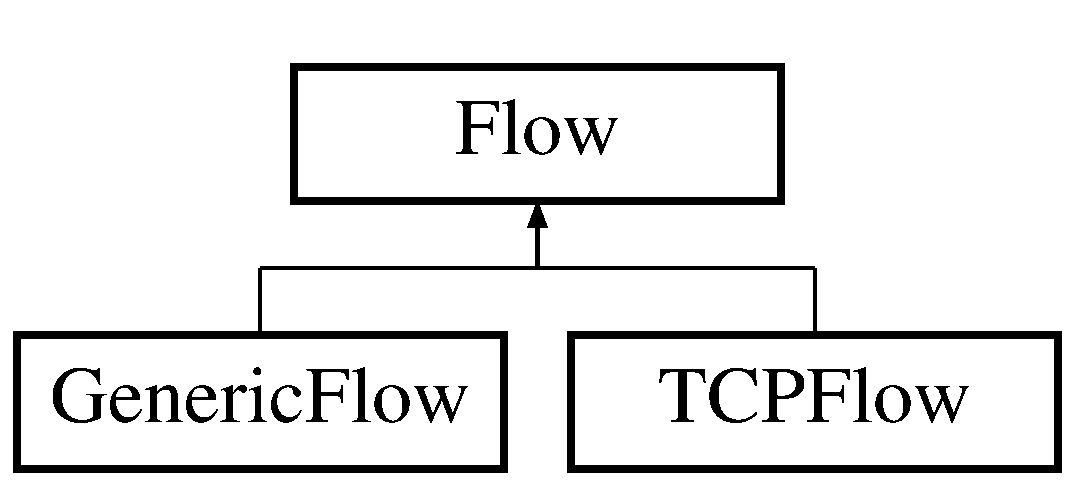
\includegraphics[height=2.000000cm]{class_flow}
\end{center}
\end{figure}
\subsection*{Public Member Functions}
\begin{DoxyCompactItemize}
\item 
virtual \hyperlink{class_flow_a5991efa6e8cf88c4ef2125cc727db333}{$\sim$\+Flow} ()
\item 
virtual bool \hyperlink{class_flow_aabcb243e3a9c04c1eb9b1090a3520544}{handle\+Packet} (Crafter\+::\+Packet $\ast$)=0
\item 
const \hyperlink{class_flow}{Flow} $\ast$ \hyperlink{class_flow_a30c028250e76e2c76837b19791185733}{get\+Brother} () const 
\item 
void \hyperlink{class_flow_ac41cf6542a8ef14cae38ed131d34dbb9}{set\+Brother} (\hyperlink{class_flow}{Flow} $\ast$\hyperlink{class_flow_aa8076d1b48c6de5c736bc64164d15320}{brother})
\end{DoxyCompactItemize}
\subsection*{Static Public Member Functions}
\begin{DoxyCompactItemize}
\item 
static std\+::pair$<$ \hyperlink{class_flow}{Flow} $\ast$, \hyperlink{class_flow}{Flow} $\ast$ $>$ $\ast$ \hyperlink{class_flow_aa3e211d010942314d8811879bb87e191}{make\+Flow\+Pair} (uint8\+\_\+t, std\+::string, std\+::string)
\item 
static \hyperlink{class_flow}{Flow} $\ast$ \hyperlink{class_flow_a46a48b06f94913c9d3ea42ca16b14794}{make\+Flow} (uint8\+\_\+t, std\+::string)
\end{DoxyCompactItemize}
\subsection*{Protected Member Functions}
\begin{DoxyCompactItemize}
\item 
\hyperlink{class_flow_af268e1b04298b6c2e123a5112fb3206f}{Flow} (std\+::string \hyperlink{class_flow_a52567a3ca729f427bf869efb594723d6}{key})
\end{DoxyCompactItemize}
\subsection*{Protected Attributes}
\begin{DoxyCompactItemize}
\item 
std\+::string \hyperlink{class_flow_a52567a3ca729f427bf869efb594723d6}{key}
\item 
\hyperlink{class_flow}{Flow} $\ast$ \hyperlink{class_flow_aa8076d1b48c6de5c736bc64164d15320}{brother}
\item 
bool \hyperlink{class_flow_ae5faa5bcc061f892714082b3dc199408}{modified} = false
\end{DoxyCompactItemize}


\subsection{Detailed Description}


Definition at line 37 of file Flow.\+h.



\subsection{Constructor \& Destructor Documentation}
\index{Flow@{Flow}!````~Flow@{$\sim$\+Flow}}
\index{````~Flow@{$\sim$\+Flow}!Flow@{Flow}}
\subsubsection[{\texorpdfstring{$\sim$\+Flow()}{~Flow()}}]{\setlength{\rightskip}{0pt plus 5cm}Flow\+::$\sim$\+Flow (
\begin{DoxyParamCaption}
{}
\end{DoxyParamCaption}
)\hspace{0.3cm}{\ttfamily [virtual]}}\hypertarget{class_flow_a5991efa6e8cf88c4ef2125cc727db333}{}\label{class_flow_a5991efa6e8cf88c4ef2125cc727db333}


Definition at line 34 of file Flow.\+cpp.

\index{Flow@{Flow}!Flow@{Flow}}
\index{Flow@{Flow}!Flow@{Flow}}
\subsubsection[{\texorpdfstring{Flow(std\+::string key)}{Flow(std::string key)}}]{\setlength{\rightskip}{0pt plus 5cm}Flow\+::\+Flow (
\begin{DoxyParamCaption}
\item[{std\+::string}]{key}
\end{DoxyParamCaption}
)\hspace{0.3cm}{\ttfamily [protected]}}\hypertarget{class_flow_af268e1b04298b6c2e123a5112fb3206f}{}\label{class_flow_af268e1b04298b6c2e123a5112fb3206f}


Definition at line 29 of file Flow.\+cpp.



\subsection{Member Function Documentation}
\index{Flow@{Flow}!get\+Brother@{get\+Brother}}
\index{get\+Brother@{get\+Brother}!Flow@{Flow}}
\subsubsection[{\texorpdfstring{get\+Brother() const }{getBrother() const }}]{\setlength{\rightskip}{0pt plus 5cm}const {\bf Flow}$\ast$ Flow\+::get\+Brother (
\begin{DoxyParamCaption}
{}
\end{DoxyParamCaption}
) const\hspace{0.3cm}{\ttfamily [inline]}}\hypertarget{class_flow_a30c028250e76e2c76837b19791185733}{}\label{class_flow_a30c028250e76e2c76837b19791185733}


Definition at line 58 of file Flow.\+h.

\index{Flow@{Flow}!handle\+Packet@{handle\+Packet}}
\index{handle\+Packet@{handle\+Packet}!Flow@{Flow}}
\subsubsection[{\texorpdfstring{handle\+Packet(\+Crafter\+::\+Packet $\ast$)=0}{handlePacket(Crafter::Packet *)=0}}]{\setlength{\rightskip}{0pt plus 5cm}virtual bool Flow\+::handle\+Packet (
\begin{DoxyParamCaption}
\item[{Crafter\+::\+Packet $\ast$}]{}
\end{DoxyParamCaption}
)\hspace{0.3cm}{\ttfamily [pure virtual]}}\hypertarget{class_flow_aabcb243e3a9c04c1eb9b1090a3520544}{}\label{class_flow_aabcb243e3a9c04c1eb9b1090a3520544}
Interface to be implemented by sibling classes. 

Implemented in \hyperlink{class_generic_flow_a5c859935f4af3f4fd2754be1c31086c8}{Generic\+Flow}, and \hyperlink{class_t_c_p_flow_a3ff0dd52eb3f3660dcb092d47da1b2f5}{T\+C\+P\+Flow}.

\index{Flow@{Flow}!make\+Flow@{make\+Flow}}
\index{make\+Flow@{make\+Flow}!Flow@{Flow}}
\subsubsection[{\texorpdfstring{make\+Flow(uint8\+\_\+t, std\+::string)}{makeFlow(uint8_t, std::string)}}]{\setlength{\rightskip}{0pt plus 5cm}{\bf Flow} $\ast$ Flow\+::make\+Flow (
\begin{DoxyParamCaption}
\item[{uint8\+\_\+t}]{protocol\+\_\+id, }
\item[{std\+::string}]{key}
\end{DoxyParamCaption}
)\hspace{0.3cm}{\ttfamily [static]}}\hypertarget{class_flow_a46a48b06f94913c9d3ea42ca16b14794}{}\label{class_flow_a46a48b06f94913c9d3ea42ca16b14794}
Fix\+ME\+: this should not be here.\+Maybe... It should not know about sibling classes ?? This is a factory method that creates a flow a generated key. 

Definition at line 56 of file Flow.\+cpp.

\index{Flow@{Flow}!make\+Flow\+Pair@{make\+Flow\+Pair}}
\index{make\+Flow\+Pair@{make\+Flow\+Pair}!Flow@{Flow}}
\subsubsection[{\texorpdfstring{make\+Flow\+Pair(uint8\+\_\+t, std\+::string, std\+::string)}{makeFlowPair(uint8_t, std::string, std::string)}}]{\setlength{\rightskip}{0pt plus 5cm}std\+::pair$<$ {\bf Flow} $\ast$, {\bf Flow} $\ast$ $>$ $\ast$ Flow\+::make\+Flow\+Pair (
\begin{DoxyParamCaption}
\item[{uint8\+\_\+t}]{protocol\+\_\+id, }
\item[{std\+::string}]{key0, }
\item[{std\+::string}]{key1}
\end{DoxyParamCaption}
)\hspace{0.3cm}{\ttfamily [static]}}\hypertarget{class_flow_aa3e211d010942314d8811879bb87e191}{}\label{class_flow_aa3e211d010942314d8811879bb87e191}
Class that representing a communication channel. Fix\+ME\+: this should not be here. Maybe... It should not know about sibling classes ?? This is a factory method that creates both flow pairs for two generated keys. 

Definition at line 38 of file Flow.\+cpp.

\index{Flow@{Flow}!set\+Brother@{set\+Brother}}
\index{set\+Brother@{set\+Brother}!Flow@{Flow}}
\subsubsection[{\texorpdfstring{set\+Brother(\+Flow $\ast$brother)}{setBrother(Flow *brother)}}]{\setlength{\rightskip}{0pt plus 5cm}void Flow\+::set\+Brother (
\begin{DoxyParamCaption}
\item[{{\bf Flow} $\ast$}]{brother}
\end{DoxyParamCaption}
)\hspace{0.3cm}{\ttfamily [inline]}}\hypertarget{class_flow_ac41cf6542a8ef14cae38ed131d34dbb9}{}\label{class_flow_ac41cf6542a8ef14cae38ed131d34dbb9}


Definition at line 61 of file Flow.\+h.



\subsection{Member Data Documentation}
\index{Flow@{Flow}!brother@{brother}}
\index{brother@{brother}!Flow@{Flow}}
\subsubsection[{\texorpdfstring{brother}{brother}}]{\setlength{\rightskip}{0pt plus 5cm}{\bf Flow}$\ast$ Flow\+::brother\hspace{0.3cm}{\ttfamily [protected]}}\hypertarget{class_flow_aa8076d1b48c6de5c736bc64164d15320}{}\label{class_flow_aa8076d1b48c6de5c736bc64164d15320}


Definition at line 68 of file Flow.\+h.

\index{Flow@{Flow}!key@{key}}
\index{key@{key}!Flow@{Flow}}
\subsubsection[{\texorpdfstring{key}{key}}]{\setlength{\rightskip}{0pt plus 5cm}std\+::string Flow\+::key\hspace{0.3cm}{\ttfamily [protected]}}\hypertarget{class_flow_a52567a3ca729f427bf869efb594723d6}{}\label{class_flow_a52567a3ca729f427bf869efb594723d6}


Definition at line 67 of file Flow.\+h.

\index{Flow@{Flow}!modified@{modified}}
\index{modified@{modified}!Flow@{Flow}}
\subsubsection[{\texorpdfstring{modified}{modified}}]{\setlength{\rightskip}{0pt plus 5cm}bool Flow\+::modified = false\hspace{0.3cm}{\ttfamily [protected]}}\hypertarget{class_flow_ae5faa5bcc061f892714082b3dc199408}{}\label{class_flow_ae5faa5bcc061f892714082b3dc199408}


Definition at line 69 of file Flow.\+h.



The documentation for this class was generated from the following files\+:\begin{DoxyCompactItemize}
\item 
/home/xshell/git/\+Reht\+Se/include/flows/\hyperlink{_flow_8h}{Flow.\+h}\item 
/home/xshell/git/\+Reht\+Se/src/flows/\hyperlink{_flow_8cpp}{Flow.\+cpp}\end{DoxyCompactItemize}

\hypertarget{class_flow_tracker}{}\section{Flow\+Tracker Class Reference}
\label{class_flow_tracker}\index{Flow\+Tracker@{Flow\+Tracker}}


{\ttfamily \#include $<$Flow\+Tracker.\+h$>$}

\subsection*{Public Member Functions}
\begin{DoxyCompactItemize}
\item 
virtual \hyperlink{class_flow_tracker_a439064075c7143f0bbe90183f20d7213}{$\sim$\+Flow\+Tracker} ()
\item 
bool \hyperlink{class_flow_tracker_a8209b693ab5ad12ef22f6793f4f98deb}{handle\+Packet} (Crafter\+::\+Packet $\ast$)
\item 
void \hyperlink{class_flow_tracker_a65f7a0712c4ed35bb1ed2b7ea832c61c}{traverse} ()
\item 
\hyperlink{class_flow}{Flow} $\ast$ \hyperlink{class_flow_tracker_a4ca33cbd3d000f5378743e23bbe64b20}{get\+Flow} (std\+::string, std\+::string)
\item 
std\+::pair$<$ std\+::string, std\+::string $>$ \hyperlink{class_flow_tracker_a3f379f0ef44c9b1af4e83ca67952938b}{build\+Flow\+Key} (Crafter\+::\+IP $\ast$)
\end{DoxyCompactItemize}
\subsection*{Static Public Member Functions}
\begin{DoxyCompactItemize}
\item 
static \hyperlink{class_flow_tracker}{Flow\+Tracker} $\ast$ \hyperlink{class_flow_tracker_ad0202e9012b222ffb96eb3c108949053}{instance} ()
\end{DoxyCompactItemize}
\subsection*{Friends}
\begin{DoxyCompactItemize}
\item 
class \hyperlink{class_flow_tracker_a4f3bf5ddad62048a5ba0f424952c3e35}{Flow}
\end{DoxyCompactItemize}


\subsection{Detailed Description}


Definition at line 35 of file Flow\+Tracker.\+h.



\subsection{Constructor \& Destructor Documentation}
\index{Flow\+Tracker@{Flow\+Tracker}!````~Flow\+Tracker@{$\sim$\+Flow\+Tracker}}
\index{````~Flow\+Tracker@{$\sim$\+Flow\+Tracker}!Flow\+Tracker@{Flow\+Tracker}}
\subsubsection[{\texorpdfstring{$\sim$\+Flow\+Tracker()}{~FlowTracker()}}]{\setlength{\rightskip}{0pt plus 5cm}Flow\+Tracker\+::$\sim$\+Flow\+Tracker (
\begin{DoxyParamCaption}
{}
\end{DoxyParamCaption}
)\hspace{0.3cm}{\ttfamily [virtual]}}\hypertarget{class_flow_tracker_a439064075c7143f0bbe90183f20d7213}{}\label{class_flow_tracker_a439064075c7143f0bbe90183f20d7213}
Fix\+ME\+: I\textquotesingle{}m not releasing memory. 

Definition at line 41 of file Flow\+Tracker.\+cpp.



\subsection{Member Function Documentation}
\index{Flow\+Tracker@{Flow\+Tracker}!build\+Flow\+Key@{build\+Flow\+Key}}
\index{build\+Flow\+Key@{build\+Flow\+Key}!Flow\+Tracker@{Flow\+Tracker}}
\subsubsection[{\texorpdfstring{build\+Flow\+Key(\+Crafter\+::\+I\+P $\ast$)}{buildFlowKey(Crafter::IP *)}}]{\setlength{\rightskip}{0pt plus 5cm}std\+::pair$<$ std\+::string, std\+::string $>$ Flow\+Tracker\+::build\+Flow\+Key (
\begin{DoxyParamCaption}
\item[{Crafter\+::\+IP $\ast$}]{packet}
\end{DoxyParamCaption}
)}\hypertarget{class_flow_tracker_a3f379f0ef44c9b1af4e83ca67952938b}{}\label{class_flow_tracker_a3f379f0ef44c9b1af4e83ca67952938b}
Creates a pair of strings to be used as keys to access the radix looking for a \hyperlink{class_flow}{Flow(first)} or its brother(second) 
\begin{DoxyParams}{Parameters}
{\em Crafter\+::\+IP} & $\ast$ ip layer to build the flow key from. \\
\hline
\end{DoxyParams}
\begin{DoxyReturn}{Returns}
std\+::pair$<$std\+::string,std\+::string$>$ 
\end{DoxyReturn}


Definition at line 94 of file Flow\+Tracker.\+cpp.

\index{Flow\+Tracker@{Flow\+Tracker}!get\+Flow@{get\+Flow}}
\index{get\+Flow@{get\+Flow}!Flow\+Tracker@{Flow\+Tracker}}
\subsubsection[{\texorpdfstring{get\+Flow(std\+::string, std\+::string)}{getFlow(std::string, std::string)}}]{\setlength{\rightskip}{0pt plus 5cm}{\bf Flow} $\ast$ Flow\+Tracker\+::get\+Flow (
\begin{DoxyParamCaption}
\item[{std\+::string}]{key, }
\item[{std\+::string}]{brother\+\_\+key}
\end{DoxyParamCaption}
)}\hypertarget{class_flow_tracker_a4ca33cbd3d000f5378743e23bbe64b20}{}\label{class_flow_tracker_a4ca33cbd3d000f5378743e23bbe64b20}
Look inside the radix for the first key. If finds it returns the given \hyperlink{class_flow}{Flow}. Else creates both flow and its brother and links them. \begin{DoxyReturn}{Returns}
Flow$\ast$ contained in the radix 
\end{DoxyReturn}


Definition at line 70 of file Flow\+Tracker.\+cpp.

\index{Flow\+Tracker@{Flow\+Tracker}!handle\+Packet@{handle\+Packet}}
\index{handle\+Packet@{handle\+Packet}!Flow\+Tracker@{Flow\+Tracker}}
\subsubsection[{\texorpdfstring{handle\+Packet(\+Crafter\+::\+Packet $\ast$)}{handlePacket(Crafter::Packet *)}}]{\setlength{\rightskip}{0pt plus 5cm}bool Flow\+Tracker\+::handle\+Packet (
\begin{DoxyParamCaption}
\item[{Crafter\+::\+Packet $\ast$}]{packet}
\end{DoxyParamCaption}
)}\hypertarget{class_flow_tracker_a8209b693ab5ad12ef22f6793f4f98deb}{}\label{class_flow_tracker_a8209b693ab5ad12ef22f6793f4f98deb}
Defines the execution flow for each packet\+: 1º Create access key. 2º get\+Flow 3º flow-\/$>$handle\+Packet... \begin{DoxyReturn}{Returns}
bool. true if packet was modified at any step. 
\end{DoxyReturn}


Definition at line 58 of file Flow\+Tracker.\+cpp.

\index{Flow\+Tracker@{Flow\+Tracker}!instance@{instance}}
\index{instance@{instance}!Flow\+Tracker@{Flow\+Tracker}}
\subsubsection[{\texorpdfstring{instance()}{instance()}}]{\setlength{\rightskip}{0pt plus 5cm}{\bf Flow\+Tracker} $\ast$ Flow\+Tracker\+::instance (
\begin{DoxyParamCaption}
{}
\end{DoxyParamCaption}
)\hspace{0.3cm}{\ttfamily [static]}}\hypertarget{class_flow_tracker_ad0202e9012b222ffb96eb3c108949053}{}\label{class_flow_tracker_ad0202e9012b222ffb96eb3c108949053}
Singleton stuff \begin{DoxyReturn}{Returns}
the unique instance of this class. 
\end{DoxyReturn}


Definition at line 30 of file Flow\+Tracker.\+cpp.

\index{Flow\+Tracker@{Flow\+Tracker}!traverse@{traverse}}
\index{traverse@{traverse}!Flow\+Tracker@{Flow\+Tracker}}
\subsubsection[{\texorpdfstring{traverse()}{traverse()}}]{\setlength{\rightskip}{0pt plus 5cm}void Flow\+Tracker\+::traverse (
\begin{DoxyParamCaption}
{}
\end{DoxyParamCaption}
)}\hypertarget{class_flow_tracker_a65f7a0712c4ed35bb1ed2b7ea832c61c}{}\label{class_flow_tracker_a65f7a0712c4ed35bb1ed2b7ea832c61c}
Writes the radix tree to the console. 

Definition at line 45 of file Flow\+Tracker.\+cpp.



\subsection{Friends And Related Function Documentation}
\index{Flow\+Tracker@{Flow\+Tracker}!Flow@{Flow}}
\index{Flow@{Flow}!Flow\+Tracker@{Flow\+Tracker}}
\subsubsection[{\texorpdfstring{Flow}{Flow}}]{\setlength{\rightskip}{0pt plus 5cm}friend class {\bf Flow}\hspace{0.3cm}{\ttfamily [friend]}}\hypertarget{class_flow_tracker_a4f3bf5ddad62048a5ba0f424952c3e35}{}\label{class_flow_tracker_a4f3bf5ddad62048a5ba0f424952c3e35}
Class that manages flow creation and access each time a packet traverses this program. 

Definition at line 41 of file Flow\+Tracker.\+h.



The documentation for this class was generated from the following files\+:\begin{DoxyCompactItemize}
\item 
/home/xshell/git/\+Reht\+Se/include/flows/\hyperlink{_flow_tracker_8h}{Flow\+Tracker.\+h}\item 
/home/xshell/git/\+Reht\+Se/src/flows/\hyperlink{_flow_tracker_8cpp}{Flow\+Tracker.\+cpp}\end{DoxyCompactItemize}

\hypertarget{class_generic_flow}{}\section{Generic\+Flow Class Reference}
\label{class_generic_flow}\index{Generic\+Flow@{Generic\+Flow}}


{\ttfamily \#include $<$Generic\+Flow.\+h$>$}

Inheritance diagram for Generic\+Flow\+:\begin{figure}[H]
\begin{center}
\leavevmode
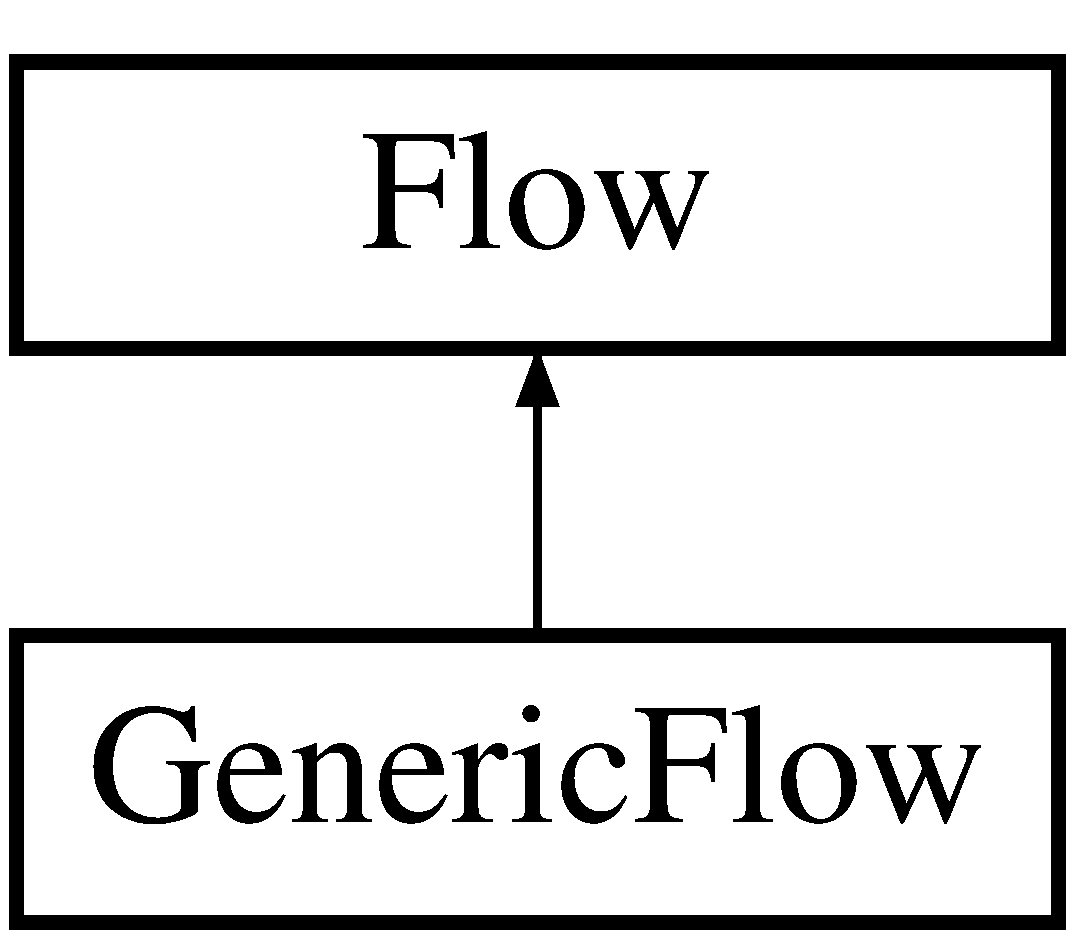
\includegraphics[height=2.000000cm]{class_generic_flow}
\end{center}
\end{figure}
\subsection*{Public Member Functions}
\begin{DoxyCompactItemize}
\item 
\hyperlink{class_generic_flow_a64cffa198c737d3e5fd3da43d6a6a0af}{Generic\+Flow} (std\+::string)
\item 
virtual \hyperlink{class_generic_flow_ae2d0e2664aa8c7196450093be73ae61a}{$\sim$\+Generic\+Flow} ()
\item 
bool \hyperlink{class_generic_flow_a5c859935f4af3f4fd2754be1c31086c8}{handle\+Packet} (Crafter\+::\+Packet $\ast$)
\end{DoxyCompactItemize}
\subsection*{Static Public Member Functions}
\begin{DoxyCompactItemize}
\item 
static void \hyperlink{class_generic_flow_a6963b91b082157c84ef967e7aa6a2fab}{update\+Key} (std\+::string \&key\+\_\+s, std\+::string \&key\+\_\+d, Crafter\+::\+IP $\ast$packet)
\end{DoxyCompactItemize}
\subsection*{Additional Inherited Members}


\subsection{Detailed Description}


Definition at line 33 of file Generic\+Flow.\+h.



\subsection{Constructor \& Destructor Documentation}
\index{Generic\+Flow@{Generic\+Flow}!Generic\+Flow@{Generic\+Flow}}
\index{Generic\+Flow@{Generic\+Flow}!Generic\+Flow@{Generic\+Flow}}
\subsubsection[{\texorpdfstring{Generic\+Flow(std\+::string)}{GenericFlow(std::string)}}]{\setlength{\rightskip}{0pt plus 5cm}Generic\+Flow\+::\+Generic\+Flow (
\begin{DoxyParamCaption}
\item[{std\+::string}]{key}
\end{DoxyParamCaption}
)}\hypertarget{class_generic_flow_a64cffa198c737d3e5fd3da43d6a6a0af}{}\label{class_generic_flow_a64cffa198c737d3e5fd3da43d6a6a0af}
Creates an instance from the key provided. 
\begin{DoxyParams}{Parameters}
{\em std\+::string} & key identifying this flow. \\
\hline
\end{DoxyParams}


Definition at line 28 of file Generic\+Flow.\+cpp.

\index{Generic\+Flow@{Generic\+Flow}!````~Generic\+Flow@{$\sim$\+Generic\+Flow}}
\index{````~Generic\+Flow@{$\sim$\+Generic\+Flow}!Generic\+Flow@{Generic\+Flow}}
\subsubsection[{\texorpdfstring{$\sim$\+Generic\+Flow()}{~GenericFlow()}}]{\setlength{\rightskip}{0pt plus 5cm}Generic\+Flow\+::$\sim$\+Generic\+Flow (
\begin{DoxyParamCaption}
{}
\end{DoxyParamCaption}
)\hspace{0.3cm}{\ttfamily [virtual]}}\hypertarget{class_generic_flow_ae2d0e2664aa8c7196450093be73ae61a}{}\label{class_generic_flow_ae2d0e2664aa8c7196450093be73ae61a}


Definition at line 31 of file Generic\+Flow.\+cpp.



\subsection{Member Function Documentation}
\index{Generic\+Flow@{Generic\+Flow}!handle\+Packet@{handle\+Packet}}
\index{handle\+Packet@{handle\+Packet}!Generic\+Flow@{Generic\+Flow}}
\subsubsection[{\texorpdfstring{handle\+Packet(\+Crafter\+::\+Packet $\ast$)}{handlePacket(Crafter::Packet *)}}]{\setlength{\rightskip}{0pt plus 5cm}bool Generic\+Flow\+::handle\+Packet (
\begin{DoxyParamCaption}
\item[{Crafter\+::\+Packet $\ast$}]{packet}
\end{DoxyParamCaption}
)\hspace{0.3cm}{\ttfamily [virtual]}}\hypertarget{class_generic_flow_a5c859935f4af3f4fd2754be1c31086c8}{}\label{class_generic_flow_a5c859935f4af3f4fd2754be1c31086c8}
Implements the most generic modification flow. If matches, then change and dispatch. Fix\+ME\+:¿¿¿\+The flow is marked as modified and further packets will be crafted again anyway. ??? 
\begin{DoxyParams}{Parameters}
{\em Crafter\+::\+Packet$\ast$} & to be handled. This object may be modified. \\
\hline
\end{DoxyParams}
\begin{DoxyReturn}{Returns}
bool. True if packet was modified. 
\end{DoxyReturn}


Implements \hyperlink{class_flow_aabcb243e3a9c04c1eb9b1090a3520544}{Flow}.



Definition at line 34 of file Generic\+Flow.\+cpp.

\index{Generic\+Flow@{Generic\+Flow}!update\+Key@{update\+Key}}
\index{update\+Key@{update\+Key}!Generic\+Flow@{Generic\+Flow}}
\subsubsection[{\texorpdfstring{update\+Key(std\+::string \&key\+\_\+s, std\+::string \&key\+\_\+d, Crafter\+::\+I\+P $\ast$packet)}{updateKey(std::string &key_s, std::string &key_d, Crafter::IP *packet)}}]{\setlength{\rightskip}{0pt plus 5cm}void Generic\+Flow\+::update\+Key (
\begin{DoxyParamCaption}
\item[{std\+::string \&}]{key\+\_\+s, }
\item[{std\+::string \&}]{key\+\_\+d, }
\item[{Crafter\+::\+IP $\ast$}]{packet}
\end{DoxyParamCaption}
)\hspace{0.3cm}{\ttfamily [static]}}\hypertarget{class_generic_flow_a6963b91b082157c84ef967e7aa6a2fab}{}\label{class_generic_flow_a6963b91b082157c84ef967e7aa6a2fab}
Class representing a \hyperlink{class_generic_flow}{Generic\+Flow} of information. It does not consider any facts related to connection oriented protocols. Generates keys considering first byte pair \mbox{[}0,1\mbox{]} as sport and the second one \mbox{[}2,3\mbox{]} as dport. Updates content of strings given as parameter. 
\begin{DoxyParams}{Parameters}
{\em std\+::string} & \& key source direct multiplexing key \\
\hline
{\em std\+::string} & \& key destination opposite multiplexing key \\
\hline
{\em Crafter\+::\+I\+P$\ast$} & packet packet to take data from \\
\hline
\end{DoxyParams}


Definition at line 57 of file Generic\+Flow.\+cpp.



The documentation for this class was generated from the following files\+:\begin{DoxyCompactItemize}
\item 
/home/xshell/git/\+Reht\+Se/include/flows/\hyperlink{_generic_flow_8h}{Generic\+Flow.\+h}\item 
/home/xshell/git/\+Reht\+Se/src/flows/\hyperlink{_generic_flow_8cpp}{Generic\+Flow.\+cpp}\end{DoxyCompactItemize}

\hypertarget{structnfq__data}{}\section{nfq\+\_\+data Struct Reference}
\label{structnfq__data}\index{nfq\+\_\+data@{nfq\+\_\+data}}


{\ttfamily \#include $<$N\+F\+Queue.\+h$>$}

\subsection*{Public Attributes}
\begin{DoxyCompactItemize}
\item 
struct nfattr $\ast$$\ast$ \hyperlink{structnfq__data_ac44f5e55ab31da6358aed4691f76a646}{data}
\end{DoxyCompactItemize}


\subsection{Detailed Description}


Definition at line 33 of file N\+F\+Queue.\+h.



\subsection{Member Data Documentation}
\index{nfq\+\_\+data@{nfq\+\_\+data}!data@{data}}
\index{data@{data}!nfq\+\_\+data@{nfq\+\_\+data}}
\subsubsection[{\texorpdfstring{data}{data}}]{\setlength{\rightskip}{0pt plus 5cm}struct nfattr$\ast$$\ast$ nfq\+\_\+data\+::data}\hypertarget{structnfq__data_ac44f5e55ab31da6358aed4691f76a646}{}\label{structnfq__data_ac44f5e55ab31da6358aed4691f76a646}


Definition at line 34 of file N\+F\+Queue.\+h.



The documentation for this struct was generated from the following file\+:\begin{DoxyCompactItemize}
\item 
/home/xshell/git/\+Reht\+Se/include/\hyperlink{_n_f_queue_8h}{N\+F\+Queue.\+h}\end{DoxyCompactItemize}

\hypertarget{class_n_f_queue}{}\section{N\+F\+Queue Class Reference}
\label{class_n_f_queue}\index{N\+F\+Queue@{N\+F\+Queue}}


{\ttfamily \#include $<$N\+F\+Queue.\+h$>$}

\subsection*{Public Member Functions}
\begin{DoxyCompactItemize}
\item 
\hyperlink{class_n_f_queue_a8fbffa750318af4d6a9323a2ab50b409}{N\+F\+Queue} (boost\+::asio\+::io\+\_\+service $\ast$)
\item 
virtual \hyperlink{class_n_f_queue_a5755ef3cf16e5a80d129f09c920a09d6}{$\sim$\+N\+F\+Queue} ()
\item 
void \hyperlink{class_n_f_queue_af92f81186532c755361d278f423d4bfb}{async\+\_\+process\+\_\+netfilterqueue\+\_\+packet} ()
\end{DoxyCompactItemize}
\subsection*{Public Attributes}
\begin{DoxyCompactItemize}
\item 
boost\+::asio\+::io\+\_\+service $\ast$ \hyperlink{class_n_f_queue_acebef7ff7290fbadb7fd04ff3075130c}{ios}
\end{DoxyCompactItemize}


\subsection{Detailed Description}


Definition at line 41 of file N\+F\+Queue.\+h.



\subsection{Constructor \& Destructor Documentation}
\index{N\+F\+Queue@{N\+F\+Queue}!N\+F\+Queue@{N\+F\+Queue}}
\index{N\+F\+Queue@{N\+F\+Queue}!N\+F\+Queue@{N\+F\+Queue}}
\subsubsection[{\texorpdfstring{N\+F\+Queue(boost\+::asio\+::io\+\_\+service $\ast$)}{NFQueue(boost::asio::io_service *)}}]{\setlength{\rightskip}{0pt plus 5cm}N\+F\+Queue\+::\+N\+F\+Queue (
\begin{DoxyParamCaption}
\item[{boost\+::asio\+::io\+\_\+service $\ast$}]{ioservice}
\end{DoxyParamCaption}
)}\hypertarget{class_n_f_queue_a8fbffa750318af4d6a9323a2ab50b409}{}\label{class_n_f_queue_a8fbffa750318af4d6a9323a2ab50b409}
\hyperlink{class_n_f_queue_a8fbffa750318af4d6a9323a2ab50b409}{N\+F\+Queue()} Perform necessary operations to register the queue. 
\begin{DoxyParams}{Parameters}
{\em boost\+::asio\+::io\+\_\+service$\ast$} & \\
\hline
\end{DoxyParams}


Definition at line 28 of file N\+F\+Queue.\+cpp.

\index{N\+F\+Queue@{N\+F\+Queue}!````~N\+F\+Queue@{$\sim$\+N\+F\+Queue}}
\index{````~N\+F\+Queue@{$\sim$\+N\+F\+Queue}!N\+F\+Queue@{N\+F\+Queue}}
\subsubsection[{\texorpdfstring{$\sim$\+N\+F\+Queue()}{~NFQueue()}}]{\setlength{\rightskip}{0pt plus 5cm}N\+F\+Queue\+::$\sim$\+N\+F\+Queue (
\begin{DoxyParamCaption}
{}
\end{DoxyParamCaption}
)\hspace{0.3cm}{\ttfamily [virtual]}}\hypertarget{class_n_f_queue_a5755ef3cf16e5a80d129f09c920a09d6}{}\label{class_n_f_queue_a5755ef3cf16e5a80d129f09c920a09d6}
Destroys the queue. 

Definition at line 66 of file N\+F\+Queue.\+cpp.



\subsection{Member Function Documentation}
\index{N\+F\+Queue@{N\+F\+Queue}!async\+\_\+process\+\_\+netfilterqueue\+\_\+packet@{async\+\_\+process\+\_\+netfilterqueue\+\_\+packet}}
\index{async\+\_\+process\+\_\+netfilterqueue\+\_\+packet@{async\+\_\+process\+\_\+netfilterqueue\+\_\+packet}!N\+F\+Queue@{N\+F\+Queue}}
\subsubsection[{\texorpdfstring{async\+\_\+process\+\_\+netfilterqueue\+\_\+packet()}{async_process_netfilterqueue_packet()}}]{\setlength{\rightskip}{0pt plus 5cm}void N\+F\+Queue\+::async\+\_\+process\+\_\+netfilterqueue\+\_\+packet (
\begin{DoxyParamCaption}
{}
\end{DoxyParamCaption}
)}\hypertarget{class_n_f_queue_af92f81186532c755361d278f423d4bfb}{}\label{class_n_f_queue_af92f81186532c755361d278f423d4bfb}
Dispatch the packet to the \hyperlink{class_flow_tracker}{Flow\+Tracker}. 

Definition at line 69 of file N\+F\+Queue.\+cpp.



\subsection{Member Data Documentation}
\index{N\+F\+Queue@{N\+F\+Queue}!ios@{ios}}
\index{ios@{ios}!N\+F\+Queue@{N\+F\+Queue}}
\subsubsection[{\texorpdfstring{ios}{ios}}]{\setlength{\rightskip}{0pt plus 5cm}boost\+::asio\+::io\+\_\+service$\ast$ N\+F\+Queue\+::ios}\hypertarget{class_n_f_queue_acebef7ff7290fbadb7fd04ff3075130c}{}\label{class_n_f_queue_acebef7ff7290fbadb7fd04ff3075130c}
Abstracts interaction with netfilter queues. 

Definition at line 46 of file N\+F\+Queue.\+h.



The documentation for this class was generated from the following files\+:\begin{DoxyCompactItemize}
\item 
/home/xshell/git/\+Reht\+Se/include/\hyperlink{_n_f_queue_8h}{N\+F\+Queue.\+h}\item 
/home/xshell/git/\+Reht\+Se/src/\hyperlink{_n_f_queue_8cpp}{N\+F\+Queue.\+cpp}\end{DoxyCompactItemize}

\hypertarget{class_pattern}{}\section{Pattern Class Reference}
\label{class_pattern}\index{Pattern@{Pattern}}


{\ttfamily \#include $<$Pattern.\+h$>$}

\subsection*{Public Member Functions}
\begin{DoxyCompactItemize}
\item 
\hyperlink{class_pattern_a7d6f58ea6e73e4b79a7f722a59ce64af}{Pattern} (std\+::string, std\+::string, std\+::string, std\+::string)
\item 
\hyperlink{class_pattern_ae0acce75099bf7776feab7d86f34e21f}{Pattern} (boost\+::property\+\_\+tree\+::ptree)
\item 
bool \hyperlink{class_pattern_a9b89524b05dc9430bd479928d4c08a4d}{check} (Crafter\+::\+Packet $\ast$)
\item 
virtual \hyperlink{class_pattern_a6e8b9388bbd39934e9f9534b974d7498}{$\sim$\+Pattern} ()
\item 
std\+::string \hyperlink{class_pattern_af1563aeb5e7bb378e810267da623906e}{print} ()
\item 
int32\+\_\+t \hyperlink{class_pattern_ac18d670fe54682f7fc6e3da229988ca0}{apply\+Replacement} (Crafter\+::\+Layer $\ast$)
\end{DoxyCompactItemize}


\subsection{Detailed Description}


Definition at line 38 of file Pattern.\+h.



\subsection{Constructor \& Destructor Documentation}
\index{Pattern@{Pattern}!Pattern@{Pattern}}
\index{Pattern@{Pattern}!Pattern@{Pattern}}
\subsubsection[{\texorpdfstring{Pattern(std\+::string, std\+::string, std\+::string, std\+::string)}{Pattern(std::string, std::string, std::string, std::string)}}]{\setlength{\rightskip}{0pt plus 5cm}Pattern\+::\+Pattern (
\begin{DoxyParamCaption}
\item[{std\+::string}]{bpf, }
\item[{std\+::string}]{regex, }
\item[{std\+::string}]{replacement\+\_\+regex, }
\item[{std\+::string}]{raw\+\_\+replacement}
\end{DoxyParamCaption}
)}\hypertarget{class_pattern_a7d6f58ea6e73e4b79a7f722a59ce64af}{}\label{class_pattern_a7d6f58ea6e73e4b79a7f722a59ce64af}
Class that implements a \hyperlink{class_pattern}{Pattern}. A pattern is composed by\+: B\+PF filter Regex Plus some replacement stuff that fits the operations for what this program is thought to be. Replacement is composed by a regex and a replacement string. Constructs a pattern from\+: bpf\+\_\+string(bpf), regex(regex), replacement\+\_\+regex(replacement\+\_\+regex), raw\+\_\+replacement(raw\+\_\+replacement) It compiles the bpf program and regex. Raises\+: B\+P\+F\+\_\+\+E\+RR if cannot compile the filter. 
\begin{DoxyParams}{Parameters}
{\em std\+::string} & bpf filter string. \\
\hline
{\em std\+::string} & regex to match packets against \\
\hline
{\em std\+::string} & regex to replace content \\
\hline
{\em std\+::string} & replacement string \\
\hline
\end{DoxyParams}


Definition at line 28 of file Pattern.\+cpp.

\index{Pattern@{Pattern}!Pattern@{Pattern}}
\index{Pattern@{Pattern}!Pattern@{Pattern}}
\subsubsection[{\texorpdfstring{Pattern(boost\+::property\+\_\+tree\+::ptree)}{Pattern(boost::property_tree::ptree)}}]{\setlength{\rightskip}{0pt plus 5cm}Pattern\+::\+Pattern (
\begin{DoxyParamCaption}
\item[{boost\+::property\+\_\+tree\+::ptree}]{ptree}
\end{DoxyParamCaption}
)}\hypertarget{class_pattern_ae0acce75099bf7776feab7d86f34e21f}{}\label{class_pattern_ae0acce75099bf7776feab7d86f34e21f}
Constructs a pattern from ptree (directly from config file). It compiles the bpf program and regex. Raises\+: B\+P\+F\+\_\+\+E\+RR if cannot compile the filter. 
\begin{DoxyParams}{Parameters}
{\em boost\+::property\+\_\+tree\+::ptree} & to create the object from. \\
\hline
\end{DoxyParams}


Definition at line 47 of file Pattern.\+cpp.

\index{Pattern@{Pattern}!````~Pattern@{$\sim$\+Pattern}}
\index{````~Pattern@{$\sim$\+Pattern}!Pattern@{Pattern}}
\subsubsection[{\texorpdfstring{$\sim$\+Pattern()}{~Pattern()}}]{\setlength{\rightskip}{0pt plus 5cm}Pattern\+::$\sim$\+Pattern (
\begin{DoxyParamCaption}
{}
\end{DoxyParamCaption}
)\hspace{0.3cm}{\ttfamily [virtual]}}\hypertarget{class_pattern_a6e8b9388bbd39934e9f9534b974d7498}{}\label{class_pattern_a6e8b9388bbd39934e9f9534b974d7498}


Definition at line 56 of file Pattern.\+cpp.



\subsection{Member Function Documentation}
\index{Pattern@{Pattern}!apply\+Replacement@{apply\+Replacement}}
\index{apply\+Replacement@{apply\+Replacement}!Pattern@{Pattern}}
\subsubsection[{\texorpdfstring{apply\+Replacement(\+Crafter\+::\+Layer $\ast$)}{applyReplacement(Crafter::Layer *)}}]{\setlength{\rightskip}{0pt plus 5cm}int32\+\_\+t Pattern\+::apply\+Replacement (
\begin{DoxyParamCaption}
\item[{Crafter\+::\+Layer $\ast$}]{layer}
\end{DoxyParamCaption}
)}\hypertarget{class_pattern_ac18d670fe54682f7fc6e3da229988ca0}{}\label{class_pattern_ac18d670fe54682f7fc6e3da229988ca0}
Apply replacement regex over the given layer. 
\begin{DoxyParams}{Parameters}
{\em Crafter\+::\+Layer} & $\ast$ over what the replacement will be applied \\
\hline
\end{DoxyParams}
\begin{DoxyReturn}{Returns}
int32\+\_\+t meaning the bytes balance\+: $>$0 if added data $<$0 if replaced data is smaller than the provided one 
\end{DoxyReturn}


Definition at line 97 of file Pattern.\+cpp.

\index{Pattern@{Pattern}!check@{check}}
\index{check@{check}!Pattern@{Pattern}}
\subsubsection[{\texorpdfstring{check(\+Crafter\+::\+Packet $\ast$)}{check(Crafter::Packet *)}}]{\setlength{\rightskip}{0pt plus 5cm}bool Pattern\+::check (
\begin{DoxyParamCaption}
\item[{Crafter\+::\+Packet $\ast$}]{packet}
\end{DoxyParamCaption}
)}\hypertarget{class_pattern_a9b89524b05dc9430bd479928d4c08a4d}{}\label{class_pattern_a9b89524b05dc9430bd479928d4c08a4d}
Checks if the packet matches the given B\+PF program and regex. 
\begin{DoxyParams}{Parameters}
{\em Crafter\+::\+Packet} & $\ast$ to be checked for matching this pattern. \\
\hline
\end{DoxyParams}


Definition at line 62 of file Pattern.\+cpp.

\index{Pattern@{Pattern}!print@{print}}
\index{print@{print}!Pattern@{Pattern}}
\subsubsection[{\texorpdfstring{print()}{print()}}]{\setlength{\rightskip}{0pt plus 5cm}std\+::string Pattern\+::print (
\begin{DoxyParamCaption}
{}
\end{DoxyParamCaption}
)\hspace{0.3cm}{\ttfamily [inline]}}\hypertarget{class_pattern_af1563aeb5e7bb378e810267da623906e}{}\label{class_pattern_af1563aeb5e7bb378e810267da623906e}
Writes printable parts of itself to a string. 

Definition at line 81 of file Pattern.\+h.



The documentation for this class was generated from the following files\+:\begin{DoxyCompactItemize}
\item 
/home/xshell/git/\+Reht\+Se/include/pattern/\hyperlink{_pattern_8h}{Pattern.\+h}\item 
/home/xshell/git/\+Reht\+Se/src/pattern/\hyperlink{_pattern_8cpp}{Pattern.\+cpp}\end{DoxyCompactItemize}

\hypertarget{classradix__tree}{}\section{radix\+\_\+tree$<$ K, T $>$ Class Template Reference}
\label{classradix__tree}\index{radix\+\_\+tree$<$ K, T $>$@{radix\+\_\+tree$<$ K, T $>$}}


{\ttfamily \#include $<$radix\+\_\+tree.\+hpp$>$}

\subsection*{Public Types}
\begin{DoxyCompactItemize}
\item 
typedef K \hyperlink{classradix__tree_a9c91791a795ceee58a0c691a46956e8a}{key\+\_\+type}
\item 
typedef T \hyperlink{classradix__tree_a08a4d9146274d8f166604a9ba670227d}{mapped\+\_\+type}
\item 
typedef std\+::pair$<$ const K, T $>$ \hyperlink{classradix__tree_a6053e1b2ccac54f990d6377a1797ebc8}{value\+\_\+type}
\item 
typedef \hyperlink{classradix__tree__it}{radix\+\_\+tree\+\_\+it}$<$ K, T $>$ \hyperlink{classradix__tree_a820fe40af6049993760c529e918c5575}{iterator}
\item 
typedef std\+::size\+\_\+t \hyperlink{classradix__tree_a67d23e7c48875261141f6259ade40749}{size\+\_\+type}
\end{DoxyCompactItemize}
\subsection*{Public Member Functions}
\begin{DoxyCompactItemize}
\item 
\hyperlink{classradix__tree_af48f519c2190b3ca6762a2d8d4bb0fb8}{radix\+\_\+tree} ()
\item 
\hyperlink{classradix__tree_a2bb7871a53afe5f826b3ab77fe039075}{$\sim$radix\+\_\+tree} ()
\item 
\hyperlink{classradix__tree_a67d23e7c48875261141f6259ade40749}{size\+\_\+type} \hyperlink{classradix__tree_aaf72ee1826a0ace064ed5f1d62f10aff}{size} () const 
\item 
bool \hyperlink{classradix__tree_ad4cdb29807c357f41ead6a4da8fd0666}{empty} () const 
\item 
void \hyperlink{classradix__tree_a6c1152cdbae47781da0f9939f32760c4}{clear} ()
\item 
\hyperlink{classradix__tree_a820fe40af6049993760c529e918c5575}{iterator} \hyperlink{classradix__tree_ac81a340d1ba443a074dfcb6cd94e10ae}{find} (const K \&key)
\item 
\hyperlink{classradix__tree_a820fe40af6049993760c529e918c5575}{iterator} \hyperlink{classradix__tree_a21d97262afed8dc8bed0d1f1059a9c5e}{begin} ()
\item 
\hyperlink{classradix__tree_a820fe40af6049993760c529e918c5575}{iterator} \hyperlink{classradix__tree_ae4f5d38cb6294fbf194eea9083fb653c}{end} ()
\item 
std\+::pair$<$ \hyperlink{classradix__tree_a820fe40af6049993760c529e918c5575}{iterator}, bool $>$ \hyperlink{classradix__tree_a6f13485d5e3091ba26fe0b51cfd49f0a}{insert} (const \hyperlink{classradix__tree_a6053e1b2ccac54f990d6377a1797ebc8}{value\+\_\+type} \&val)
\item 
bool \hyperlink{classradix__tree_a0cb893a83d6178476627810ae753a0a2}{erase} (const K \&key)
\item 
void \hyperlink{classradix__tree_a6214bf995a2f7cc3a8bd2be38bc381eb}{erase} (\hyperlink{classradix__tree_a820fe40af6049993760c529e918c5575}{iterator} it)
\item 
void \hyperlink{classradix__tree_a819af474517e7398ba61c0f72e4fa545}{prefix\+\_\+match} (const K \&key, std\+::vector$<$ \hyperlink{classradix__tree_a820fe40af6049993760c529e918c5575}{iterator} $>$ \&vec)
\item 
void \hyperlink{classradix__tree_a7fb4e244818ad60f4bbf936533ba18e1}{greedy\+\_\+match} (const K \&key, std\+::vector$<$ \hyperlink{classradix__tree_a820fe40af6049993760c529e918c5575}{iterator} $>$ \&vec)
\item 
\hyperlink{classradix__tree_a820fe40af6049993760c529e918c5575}{iterator} \hyperlink{classradix__tree_a65818f8ce51e27448a8afd47971e984e}{longest\+\_\+match} (const K \&key)
\item 
T \& \hyperlink{classradix__tree_ae66624c974244381c917486275b47738}{operator\mbox{[}$\,$\mbox{]}} (const K \&lhs)
\end{DoxyCompactItemize}


\subsection{Detailed Description}
\subsubsection*{template$<$typename K, typename T$>$\\*
class radix\+\_\+tree$<$ K, T $>$}



Definition at line 40 of file radix\+\_\+tree.\+hpp.



\subsection{Member Typedef Documentation}
\index{radix\+\_\+tree@{radix\+\_\+tree}!iterator@{iterator}}
\index{iterator@{iterator}!radix\+\_\+tree@{radix\+\_\+tree}}
\subsubsection[{\texorpdfstring{iterator}{iterator}}]{\setlength{\rightskip}{0pt plus 5cm}template$<$typename K, typename T$>$ typedef {\bf radix\+\_\+tree\+\_\+it}$<$K, T$>$ {\bf radix\+\_\+tree}$<$ K, T $>$\+::{\bf iterator}}\hypertarget{classradix__tree_a820fe40af6049993760c529e918c5575}{}\label{classradix__tree_a820fe40af6049993760c529e918c5575}


Definition at line 45 of file radix\+\_\+tree.\+hpp.

\index{radix\+\_\+tree@{radix\+\_\+tree}!key\+\_\+type@{key\+\_\+type}}
\index{key\+\_\+type@{key\+\_\+type}!radix\+\_\+tree@{radix\+\_\+tree}}
\subsubsection[{\texorpdfstring{key\+\_\+type}{key_type}}]{\setlength{\rightskip}{0pt plus 5cm}template$<$typename K, typename T$>$ typedef K {\bf radix\+\_\+tree}$<$ K, T $>$\+::{\bf key\+\_\+type}}\hypertarget{classradix__tree_a9c91791a795ceee58a0c691a46956e8a}{}\label{classradix__tree_a9c91791a795ceee58a0c691a46956e8a}


Definition at line 42 of file radix\+\_\+tree.\+hpp.

\index{radix\+\_\+tree@{radix\+\_\+tree}!mapped\+\_\+type@{mapped\+\_\+type}}
\index{mapped\+\_\+type@{mapped\+\_\+type}!radix\+\_\+tree@{radix\+\_\+tree}}
\subsubsection[{\texorpdfstring{mapped\+\_\+type}{mapped_type}}]{\setlength{\rightskip}{0pt plus 5cm}template$<$typename K, typename T$>$ typedef T {\bf radix\+\_\+tree}$<$ K, T $>$\+::{\bf mapped\+\_\+type}}\hypertarget{classradix__tree_a08a4d9146274d8f166604a9ba670227d}{}\label{classradix__tree_a08a4d9146274d8f166604a9ba670227d}


Definition at line 43 of file radix\+\_\+tree.\+hpp.

\index{radix\+\_\+tree@{radix\+\_\+tree}!size\+\_\+type@{size\+\_\+type}}
\index{size\+\_\+type@{size\+\_\+type}!radix\+\_\+tree@{radix\+\_\+tree}}
\subsubsection[{\texorpdfstring{size\+\_\+type}{size_type}}]{\setlength{\rightskip}{0pt plus 5cm}template$<$typename K, typename T$>$ typedef std\+::size\+\_\+t {\bf radix\+\_\+tree}$<$ K, T $>$\+::{\bf size\+\_\+type}}\hypertarget{classradix__tree_a67d23e7c48875261141f6259ade40749}{}\label{classradix__tree_a67d23e7c48875261141f6259ade40749}


Definition at line 46 of file radix\+\_\+tree.\+hpp.

\index{radix\+\_\+tree@{radix\+\_\+tree}!value\+\_\+type@{value\+\_\+type}}
\index{value\+\_\+type@{value\+\_\+type}!radix\+\_\+tree@{radix\+\_\+tree}}
\subsubsection[{\texorpdfstring{value\+\_\+type}{value_type}}]{\setlength{\rightskip}{0pt plus 5cm}template$<$typename K, typename T$>$ typedef std\+::pair$<$const K, T$>$ {\bf radix\+\_\+tree}$<$ K, T $>$\+::{\bf value\+\_\+type}}\hypertarget{classradix__tree_a6053e1b2ccac54f990d6377a1797ebc8}{}\label{classradix__tree_a6053e1b2ccac54f990d6377a1797ebc8}


Definition at line 44 of file radix\+\_\+tree.\+hpp.



\subsection{Constructor \& Destructor Documentation}
\index{radix\+\_\+tree@{radix\+\_\+tree}!radix\+\_\+tree@{radix\+\_\+tree}}
\index{radix\+\_\+tree@{radix\+\_\+tree}!radix\+\_\+tree@{radix\+\_\+tree}}
\subsubsection[{\texorpdfstring{radix\+\_\+tree()}{radix_tree()}}]{\setlength{\rightskip}{0pt plus 5cm}template$<$typename K, typename T$>$ {\bf radix\+\_\+tree}$<$ K, T $>$\+::{\bf radix\+\_\+tree} (
\begin{DoxyParamCaption}
{}
\end{DoxyParamCaption}
)\hspace{0.3cm}{\ttfamily [inline]}}\hypertarget{classradix__tree_af48f519c2190b3ca6762a2d8d4bb0fb8}{}\label{classradix__tree_af48f519c2190b3ca6762a2d8d4bb0fb8}


Definition at line 48 of file radix\+\_\+tree.\+hpp.

\index{radix\+\_\+tree@{radix\+\_\+tree}!````~radix\+\_\+tree@{$\sim$radix\+\_\+tree}}
\index{````~radix\+\_\+tree@{$\sim$radix\+\_\+tree}!radix\+\_\+tree@{radix\+\_\+tree}}
\subsubsection[{\texorpdfstring{$\sim$radix\+\_\+tree()}{~radix_tree()}}]{\setlength{\rightskip}{0pt plus 5cm}template$<$typename K, typename T$>$ {\bf radix\+\_\+tree}$<$ K, T $>$\+::$\sim${\bf radix\+\_\+tree} (
\begin{DoxyParamCaption}
{}
\end{DoxyParamCaption}
)\hspace{0.3cm}{\ttfamily [inline]}}\hypertarget{classradix__tree_a2bb7871a53afe5f826b3ab77fe039075}{}\label{classradix__tree_a2bb7871a53afe5f826b3ab77fe039075}


Definition at line 49 of file radix\+\_\+tree.\+hpp.



\subsection{Member Function Documentation}
\index{radix\+\_\+tree@{radix\+\_\+tree}!begin@{begin}}
\index{begin@{begin}!radix\+\_\+tree@{radix\+\_\+tree}}
\subsubsection[{\texorpdfstring{begin()}{begin()}}]{\setlength{\rightskip}{0pt plus 5cm}template$<$typename K , typename T $>$ {\bf radix\+\_\+tree}$<$ K, T $>$\+::{\bf iterator} {\bf radix\+\_\+tree}$<$ K, T $>$\+::begin (
\begin{DoxyParamCaption}
{}
\end{DoxyParamCaption}
)}\hypertarget{classradix__tree_a21d97262afed8dc8bed0d1f1059a9c5e}{}\label{classradix__tree_a21d97262afed8dc8bed0d1f1059a9c5e}


Definition at line 159 of file radix\+\_\+tree.\+hpp.

\index{radix\+\_\+tree@{radix\+\_\+tree}!clear@{clear}}
\index{clear@{clear}!radix\+\_\+tree@{radix\+\_\+tree}}
\subsubsection[{\texorpdfstring{clear()}{clear()}}]{\setlength{\rightskip}{0pt plus 5cm}template$<$typename K, typename T$>$ void {\bf radix\+\_\+tree}$<$ K, T $>$\+::clear (
\begin{DoxyParamCaption}
{}
\end{DoxyParamCaption}
)\hspace{0.3cm}{\ttfamily [inline]}}\hypertarget{classradix__tree_a6c1152cdbae47781da0f9939f32760c4}{}\label{classradix__tree_a6c1152cdbae47781da0f9939f32760c4}


Definition at line 59 of file radix\+\_\+tree.\+hpp.

\index{radix\+\_\+tree@{radix\+\_\+tree}!empty@{empty}}
\index{empty@{empty}!radix\+\_\+tree@{radix\+\_\+tree}}
\subsubsection[{\texorpdfstring{empty() const }{empty() const }}]{\setlength{\rightskip}{0pt plus 5cm}template$<$typename K, typename T$>$ bool {\bf radix\+\_\+tree}$<$ K, T $>$\+::empty (
\begin{DoxyParamCaption}
{}
\end{DoxyParamCaption}
) const\hspace{0.3cm}{\ttfamily [inline]}}\hypertarget{classradix__tree_ad4cdb29807c357f41ead6a4da8fd0666}{}\label{classradix__tree_ad4cdb29807c357f41ead6a4da8fd0666}


Definition at line 56 of file radix\+\_\+tree.\+hpp.

\index{radix\+\_\+tree@{radix\+\_\+tree}!end@{end}}
\index{end@{end}!radix\+\_\+tree@{radix\+\_\+tree}}
\subsubsection[{\texorpdfstring{end()}{end()}}]{\setlength{\rightskip}{0pt plus 5cm}template$<$typename K , typename T $>$ {\bf radix\+\_\+tree}$<$ K, T $>$\+::{\bf iterator} {\bf radix\+\_\+tree}$<$ K, T $>$\+::end (
\begin{DoxyParamCaption}
{}
\end{DoxyParamCaption}
)}\hypertarget{classradix__tree_ae4f5d38cb6294fbf194eea9083fb653c}{}\label{classradix__tree_ae4f5d38cb6294fbf194eea9083fb653c}


Definition at line 153 of file radix\+\_\+tree.\+hpp.

\index{radix\+\_\+tree@{radix\+\_\+tree}!erase@{erase}}
\index{erase@{erase}!radix\+\_\+tree@{radix\+\_\+tree}}
\subsubsection[{\texorpdfstring{erase(const K \&key)}{erase(const K &key)}}]{\setlength{\rightskip}{0pt plus 5cm}template$<$typename K, typename T $>$ bool {\bf radix\+\_\+tree}$<$ K, T $>$\+::erase (
\begin{DoxyParamCaption}
\item[{const K \&}]{key}
\end{DoxyParamCaption}
)}\hypertarget{classradix__tree_a0cb893a83d6178476627810ae753a0a2}{}\label{classradix__tree_a0cb893a83d6178476627810ae753a0a2}


Definition at line 242 of file radix\+\_\+tree.\+hpp.

\index{radix\+\_\+tree@{radix\+\_\+tree}!erase@{erase}}
\index{erase@{erase}!radix\+\_\+tree@{radix\+\_\+tree}}
\subsubsection[{\texorpdfstring{erase(iterator it)}{erase(iterator it)}}]{\setlength{\rightskip}{0pt plus 5cm}template$<$typename K, typename T $>$ void {\bf radix\+\_\+tree}$<$ K, T $>$\+::erase (
\begin{DoxyParamCaption}
\item[{{\bf iterator}}]{it}
\end{DoxyParamCaption}
)}\hypertarget{classradix__tree_a6214bf995a2f7cc3a8bd2be38bc381eb}{}\label{classradix__tree_a6214bf995a2f7cc3a8bd2be38bc381eb}


Definition at line 236 of file radix\+\_\+tree.\+hpp.

\index{radix\+\_\+tree@{radix\+\_\+tree}!find@{find}}
\index{find@{find}!radix\+\_\+tree@{radix\+\_\+tree}}
\subsubsection[{\texorpdfstring{find(const K \&key)}{find(const K &key)}}]{\setlength{\rightskip}{0pt plus 5cm}template$<$typename K, typename T $>$ {\bf radix\+\_\+tree}$<$ K, T $>$\+::{\bf iterator} {\bf radix\+\_\+tree}$<$ K, T $>$\+::find (
\begin{DoxyParamCaption}
\item[{const K \&}]{key}
\end{DoxyParamCaption}
)}\hypertarget{classradix__tree_ac81a340d1ba443a074dfcb6cd94e10ae}{}\label{classradix__tree_ac81a340d1ba443a074dfcb6cd94e10ae}


Definition at line 452 of file radix\+\_\+tree.\+hpp.

\index{radix\+\_\+tree@{radix\+\_\+tree}!greedy\+\_\+match@{greedy\+\_\+match}}
\index{greedy\+\_\+match@{greedy\+\_\+match}!radix\+\_\+tree@{radix\+\_\+tree}}
\subsubsection[{\texorpdfstring{greedy\+\_\+match(const K \&key, std\+::vector$<$ iterator $>$ \&vec)}{greedy_match(const K &key, std::vector< iterator > &vec)}}]{\setlength{\rightskip}{0pt plus 5cm}template$<$typename K, typename T $>$ void {\bf radix\+\_\+tree}$<$ K, T $>$\+::greedy\+\_\+match (
\begin{DoxyParamCaption}
\item[{const K \&}]{key, }
\item[{std\+::vector$<$ {\bf iterator} $>$ \&}]{vec}
\end{DoxyParamCaption}
)}\hypertarget{classradix__tree_a7fb4e244818ad60f4bbf936533ba18e1}{}\label{classradix__tree_a7fb4e244818ad60f4bbf936533ba18e1}


Definition at line 203 of file radix\+\_\+tree.\+hpp.

\index{radix\+\_\+tree@{radix\+\_\+tree}!insert@{insert}}
\index{insert@{insert}!radix\+\_\+tree@{radix\+\_\+tree}}
\subsubsection[{\texorpdfstring{insert(const value\+\_\+type \&val)}{insert(const value_type &val)}}]{\setlength{\rightskip}{0pt plus 5cm}template$<$typename K , typename T $>$ std\+::pair$<$ typename {\bf radix\+\_\+tree}$<$ K, T $>$\+::{\bf iterator}, bool $>$ {\bf radix\+\_\+tree}$<$ K, T $>$\+::insert (
\begin{DoxyParamCaption}
\item[{const {\bf value\+\_\+type} \&}]{val}
\end{DoxyParamCaption}
)}\hypertarget{classradix__tree_a6f13485d5e3091ba26fe0b51cfd49f0a}{}\label{classradix__tree_a6f13485d5e3091ba26fe0b51cfd49f0a}


Definition at line 421 of file radix\+\_\+tree.\+hpp.

\index{radix\+\_\+tree@{radix\+\_\+tree}!longest\+\_\+match@{longest\+\_\+match}}
\index{longest\+\_\+match@{longest\+\_\+match}!radix\+\_\+tree@{radix\+\_\+tree}}
\subsubsection[{\texorpdfstring{longest\+\_\+match(const K \&key)}{longest_match(const K &key)}}]{\setlength{\rightskip}{0pt plus 5cm}template$<$typename K, typename T $>$ {\bf radix\+\_\+tree}$<$ K, T $>$\+::{\bf iterator} {\bf radix\+\_\+tree}$<$ K, T $>$\+::longest\+\_\+match (
\begin{DoxyParamCaption}
\item[{const K \&}]{key}
\end{DoxyParamCaption}
)}\hypertarget{classradix__tree_a65818f8ce51e27448a8afd47971e984e}{}\label{classradix__tree_a65818f8ce51e27448a8afd47971e984e}


Definition at line 119 of file radix\+\_\+tree.\+hpp.

\index{radix\+\_\+tree@{radix\+\_\+tree}!operator\mbox{[}$\,$\mbox{]}@{operator[]}}
\index{operator\mbox{[}$\,$\mbox{]}@{operator[]}!radix\+\_\+tree@{radix\+\_\+tree}}
\subsubsection[{\texorpdfstring{operator[](const K \&lhs)}{operator[](const K &lhs)}}]{\setlength{\rightskip}{0pt plus 5cm}template$<$typename K, typename T $>$ T \& {\bf radix\+\_\+tree}$<$ K, T $>$\+::operator\mbox{[}$\,$\mbox{]} (
\begin{DoxyParamCaption}
\item[{const K \&}]{lhs}
\end{DoxyParamCaption}
)}\hypertarget{classradix__tree_ae66624c974244381c917486275b47738}{}\label{classradix__tree_ae66624c974244381c917486275b47738}


Definition at line 183 of file radix\+\_\+tree.\+hpp.

\index{radix\+\_\+tree@{radix\+\_\+tree}!prefix\+\_\+match@{prefix\+\_\+match}}
\index{prefix\+\_\+match@{prefix\+\_\+match}!radix\+\_\+tree@{radix\+\_\+tree}}
\subsubsection[{\texorpdfstring{prefix\+\_\+match(const K \&key, std\+::vector$<$ iterator $>$ \&vec)}{prefix_match(const K &key, std::vector< iterator > &vec)}}]{\setlength{\rightskip}{0pt plus 5cm}template$<$typename K, typename T $>$ void {\bf radix\+\_\+tree}$<$ K, T $>$\+::prefix\+\_\+match (
\begin{DoxyParamCaption}
\item[{const K \&}]{key, }
\item[{std\+::vector$<$ {\bf iterator} $>$ \&}]{vec}
\end{DoxyParamCaption}
)}\hypertarget{classradix__tree_a819af474517e7398ba61c0f72e4fa545}{}\label{classradix__tree_a819af474517e7398ba61c0f72e4fa545}


Definition at line 93 of file radix\+\_\+tree.\+hpp.

\index{radix\+\_\+tree@{radix\+\_\+tree}!size@{size}}
\index{size@{size}!radix\+\_\+tree@{radix\+\_\+tree}}
\subsubsection[{\texorpdfstring{size() const }{size() const }}]{\setlength{\rightskip}{0pt plus 5cm}template$<$typename K, typename T$>$ {\bf size\+\_\+type} {\bf radix\+\_\+tree}$<$ K, T $>$\+::size (
\begin{DoxyParamCaption}
{}
\end{DoxyParamCaption}
) const\hspace{0.3cm}{\ttfamily [inline]}}\hypertarget{classradix__tree_aaf72ee1826a0ace064ed5f1d62f10aff}{}\label{classradix__tree_aaf72ee1826a0ace064ed5f1d62f10aff}


Definition at line 53 of file radix\+\_\+tree.\+hpp.



The documentation for this class was generated from the following file\+:\begin{DoxyCompactItemize}
\item 
/home/xshell/git/\+Reht\+Se/include/\hyperlink{radix__tree_8hpp}{radix\+\_\+tree.\+hpp}\end{DoxyCompactItemize}

\hypertarget{classradix__tree__it}{}\section{radix\+\_\+tree\+\_\+it$<$ K, T $>$ Class Template Reference}
\label{classradix__tree__it}\index{radix\+\_\+tree\+\_\+it$<$ K, T $>$@{radix\+\_\+tree\+\_\+it$<$ K, T $>$}}


{\ttfamily \#include $<$radix\+\_\+tree\+\_\+it.\+hpp$>$}

Inheritance diagram for radix\+\_\+tree\+\_\+it$<$ K, T $>$\+:\begin{figure}[H]
\begin{center}
\leavevmode
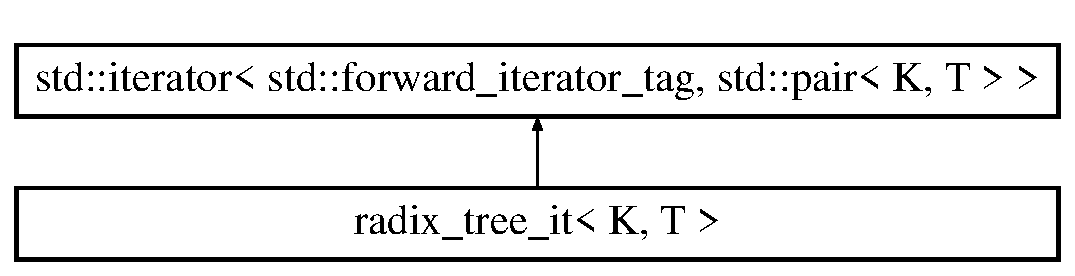
\includegraphics[height=2.000000cm]{classradix__tree__it}
\end{center}
\end{figure}
\subsection*{Public Member Functions}
\begin{DoxyCompactItemize}
\item 
\hyperlink{classradix__tree__it_ab32c43daa26d8df9031813b820bfe30f}{radix\+\_\+tree\+\_\+it} ()
\item 
\hyperlink{classradix__tree__it_a2817b4be2cc40a29a380175c9c774028}{radix\+\_\+tree\+\_\+it} (const \hyperlink{classradix__tree__it}{radix\+\_\+tree\+\_\+it} \&r)
\item 
\hyperlink{classradix__tree__it}{radix\+\_\+tree\+\_\+it} \& \hyperlink{classradix__tree__it_a2aae5ad4b5b2dacd5f77429c92fa5687}{operator=} (const \hyperlink{classradix__tree__it}{radix\+\_\+tree\+\_\+it} \&r)
\item 
\hyperlink{classradix__tree__it_a678a52ad4a84891319e79cc83046eb00}{$\sim$radix\+\_\+tree\+\_\+it} ()
\item 
std\+::pair$<$ const K, T $>$ \& \hyperlink{classradix__tree__it_ad729635bf943750c84a391adfab650d5}{operator$\ast$} () const 
\item 
std\+::pair$<$ const K, T $>$ $\ast$ \hyperlink{classradix__tree__it_af9625539926f984aea370867e96aa985}{operator-\/$>$} () const 
\item 
const \hyperlink{classradix__tree__it}{radix\+\_\+tree\+\_\+it}$<$ K, T $>$ \& \hyperlink{classradix__tree__it_aeaee75d1faafcd02ec5ff9c0fa161818}{operator++} ()
\item 
\hyperlink{classradix__tree__it}{radix\+\_\+tree\+\_\+it}$<$ K, T $>$ \hyperlink{classradix__tree__it_abd41bd4b4e1b5f7b95ec8c99030c37ae}{operator++} (int)
\item 
bool \hyperlink{classradix__tree__it_aaae533a0e6ad7b243f567798bbfdfa2b}{operator!=} (const \hyperlink{classradix__tree__it}{radix\+\_\+tree\+\_\+it}$<$ K, T $>$ \&lhs) const 
\item 
bool \hyperlink{classradix__tree__it_a0b7c9edd34bd97a360b6ca17de6b6534}{operator==} (const \hyperlink{classradix__tree__it}{radix\+\_\+tree\+\_\+it}$<$ K, T $>$ \&lhs) const 
\end{DoxyCompactItemize}
\subsection*{Friends}
\begin{DoxyCompactItemize}
\item 
class \hyperlink{classradix__tree__it_a0596aeb27884e8ff44f365527f6a8f12}{radix\+\_\+tree$<$ K, T $>$}
\end{DoxyCompactItemize}


\subsection{Detailed Description}
\subsubsection*{template$<$typename K, typename T$>$\\*
class radix\+\_\+tree\+\_\+it$<$ K, T $>$}



Definition at line 11 of file radix\+\_\+tree\+\_\+it.\+hpp.



\subsection{Constructor \& Destructor Documentation}
\index{radix\+\_\+tree\+\_\+it@{radix\+\_\+tree\+\_\+it}!radix\+\_\+tree\+\_\+it@{radix\+\_\+tree\+\_\+it}}
\index{radix\+\_\+tree\+\_\+it@{radix\+\_\+tree\+\_\+it}!radix\+\_\+tree\+\_\+it@{radix\+\_\+tree\+\_\+it}}
\subsubsection[{\texorpdfstring{radix\+\_\+tree\+\_\+it()}{radix_tree_it()}}]{\setlength{\rightskip}{0pt plus 5cm}template$<$typename K, typename T$>$ {\bf radix\+\_\+tree\+\_\+it}$<$ K, T $>$\+::{\bf radix\+\_\+tree\+\_\+it} (
\begin{DoxyParamCaption}
{}
\end{DoxyParamCaption}
)\hspace{0.3cm}{\ttfamily [inline]}}\hypertarget{classradix__tree__it_ab32c43daa26d8df9031813b820bfe30f}{}\label{classradix__tree__it_ab32c43daa26d8df9031813b820bfe30f}


Definition at line 15 of file radix\+\_\+tree\+\_\+it.\+hpp.

\index{radix\+\_\+tree\+\_\+it@{radix\+\_\+tree\+\_\+it}!radix\+\_\+tree\+\_\+it@{radix\+\_\+tree\+\_\+it}}
\index{radix\+\_\+tree\+\_\+it@{radix\+\_\+tree\+\_\+it}!radix\+\_\+tree\+\_\+it@{radix\+\_\+tree\+\_\+it}}
\subsubsection[{\texorpdfstring{radix\+\_\+tree\+\_\+it(const radix\+\_\+tree\+\_\+it \&r)}{radix_tree_it(const radix_tree_it &r)}}]{\setlength{\rightskip}{0pt plus 5cm}template$<$typename K, typename T$>$ {\bf radix\+\_\+tree\+\_\+it}$<$ K, T $>$\+::{\bf radix\+\_\+tree\+\_\+it} (
\begin{DoxyParamCaption}
\item[{const {\bf radix\+\_\+tree\+\_\+it}$<$ K, T $>$ \&}]{r}
\end{DoxyParamCaption}
)\hspace{0.3cm}{\ttfamily [inline]}}\hypertarget{classradix__tree__it_a2817b4be2cc40a29a380175c9c774028}{}\label{classradix__tree__it_a2817b4be2cc40a29a380175c9c774028}


Definition at line 16 of file radix\+\_\+tree\+\_\+it.\+hpp.

\index{radix\+\_\+tree\+\_\+it@{radix\+\_\+tree\+\_\+it}!````~radix\+\_\+tree\+\_\+it@{$\sim$radix\+\_\+tree\+\_\+it}}
\index{````~radix\+\_\+tree\+\_\+it@{$\sim$radix\+\_\+tree\+\_\+it}!radix\+\_\+tree\+\_\+it@{radix\+\_\+tree\+\_\+it}}
\subsubsection[{\texorpdfstring{$\sim$radix\+\_\+tree\+\_\+it()}{~radix_tree_it()}}]{\setlength{\rightskip}{0pt plus 5cm}template$<$typename K, typename T$>$ {\bf radix\+\_\+tree\+\_\+it}$<$ K, T $>$\+::$\sim${\bf radix\+\_\+tree\+\_\+it} (
\begin{DoxyParamCaption}
{}
\end{DoxyParamCaption}
)\hspace{0.3cm}{\ttfamily [inline]}}\hypertarget{classradix__tree__it_a678a52ad4a84891319e79cc83046eb00}{}\label{classradix__tree__it_a678a52ad4a84891319e79cc83046eb00}


Definition at line 18 of file radix\+\_\+tree\+\_\+it.\+hpp.



\subsection{Member Function Documentation}
\index{radix\+\_\+tree\+\_\+it@{radix\+\_\+tree\+\_\+it}!operator"!=@{operator"!=}}
\index{operator"!=@{operator"!=}!radix\+\_\+tree\+\_\+it@{radix\+\_\+tree\+\_\+it}}
\subsubsection[{\texorpdfstring{operator"!=(const radix\+\_\+tree\+\_\+it$<$ K, T $>$ \&lhs) const }{operator!=(const radix_tree_it< K, T > &lhs) const }}]{\setlength{\rightskip}{0pt plus 5cm}template$<$typename K , typename T $>$ bool {\bf radix\+\_\+tree\+\_\+it}$<$ K, T $>$\+::operator!= (
\begin{DoxyParamCaption}
\item[{const {\bf radix\+\_\+tree\+\_\+it}$<$ K, T $>$ \&}]{lhs}
\end{DoxyParamCaption}
) const}\hypertarget{classradix__tree__it_aaae533a0e6ad7b243f567798bbfdfa2b}{}\label{classradix__tree__it_aaae533a0e6ad7b243f567798bbfdfa2b}


Definition at line 80 of file radix\+\_\+tree\+\_\+it.\+hpp.

\index{radix\+\_\+tree\+\_\+it@{radix\+\_\+tree\+\_\+it}!operator$\ast$@{operator$\ast$}}
\index{operator$\ast$@{operator$\ast$}!radix\+\_\+tree\+\_\+it@{radix\+\_\+tree\+\_\+it}}
\subsubsection[{\texorpdfstring{operator$\ast$() const }{operator*() const }}]{\setlength{\rightskip}{0pt plus 5cm}template$<$typename K , typename T $>$ std\+::pair$<$ const K, T $>$ \& {\bf radix\+\_\+tree\+\_\+it}$<$ K, T $>$\+::operator$\ast$ (
\begin{DoxyParamCaption}
{}
\end{DoxyParamCaption}
) const}\hypertarget{classradix__tree__it_ad729635bf943750c84a391adfab650d5}{}\label{classradix__tree__it_ad729635bf943750c84a391adfab650d5}


Definition at line 68 of file radix\+\_\+tree\+\_\+it.\+hpp.

\index{radix\+\_\+tree\+\_\+it@{radix\+\_\+tree\+\_\+it}!operator++@{operator++}}
\index{operator++@{operator++}!radix\+\_\+tree\+\_\+it@{radix\+\_\+tree\+\_\+it}}
\subsubsection[{\texorpdfstring{operator++()}{operator++()}}]{\setlength{\rightskip}{0pt plus 5cm}template$<$typename K , typename T $>$ const {\bf radix\+\_\+tree\+\_\+it}$<$ K, T $>$ \& {\bf radix\+\_\+tree\+\_\+it}$<$ K, T $>$\+::operator++ (
\begin{DoxyParamCaption}
{}
\end{DoxyParamCaption}
)}\hypertarget{classradix__tree__it_aeaee75d1faafcd02ec5ff9c0fa161818}{}\label{classradix__tree__it_aeaee75d1faafcd02ec5ff9c0fa161818}


Definition at line 92 of file radix\+\_\+tree\+\_\+it.\+hpp.

\index{radix\+\_\+tree\+\_\+it@{radix\+\_\+tree\+\_\+it}!operator++@{operator++}}
\index{operator++@{operator++}!radix\+\_\+tree\+\_\+it@{radix\+\_\+tree\+\_\+it}}
\subsubsection[{\texorpdfstring{operator++(int)}{operator++(int)}}]{\setlength{\rightskip}{0pt plus 5cm}template$<$typename K , typename T $>$ {\bf radix\+\_\+tree\+\_\+it}$<$ K, T $>$ {\bf radix\+\_\+tree\+\_\+it}$<$ K, T $>$\+::operator++ (
\begin{DoxyParamCaption}
\item[{int}]{}
\end{DoxyParamCaption}
)}\hypertarget{classradix__tree__it_abd41bd4b4e1b5f7b95ec8c99030c37ae}{}\label{classradix__tree__it_abd41bd4b4e1b5f7b95ec8c99030c37ae}


Definition at line 100 of file radix\+\_\+tree\+\_\+it.\+hpp.

\index{radix\+\_\+tree\+\_\+it@{radix\+\_\+tree\+\_\+it}!operator-\/$>$@{operator-\/$>$}}
\index{operator-\/$>$@{operator-\/$>$}!radix\+\_\+tree\+\_\+it@{radix\+\_\+tree\+\_\+it}}
\subsubsection[{\texorpdfstring{operator-\/$>$() const }{operator->() const }}]{\setlength{\rightskip}{0pt plus 5cm}template$<$typename K , typename T $>$ std\+::pair$<$ const K, T $>$ $\ast$ {\bf radix\+\_\+tree\+\_\+it}$<$ K, T $>$\+::operator-\/$>$ (
\begin{DoxyParamCaption}
{}
\end{DoxyParamCaption}
) const}\hypertarget{classradix__tree__it_af9625539926f984aea370867e96aa985}{}\label{classradix__tree__it_af9625539926f984aea370867e96aa985}


Definition at line 74 of file radix\+\_\+tree\+\_\+it.\+hpp.

\index{radix\+\_\+tree\+\_\+it@{radix\+\_\+tree\+\_\+it}!operator=@{operator=}}
\index{operator=@{operator=}!radix\+\_\+tree\+\_\+it@{radix\+\_\+tree\+\_\+it}}
\subsubsection[{\texorpdfstring{operator=(const radix\+\_\+tree\+\_\+it \&r)}{operator=(const radix_tree_it &r)}}]{\setlength{\rightskip}{0pt plus 5cm}template$<$typename K, typename T$>$ {\bf radix\+\_\+tree\+\_\+it}\& {\bf radix\+\_\+tree\+\_\+it}$<$ K, T $>$\+::operator= (
\begin{DoxyParamCaption}
\item[{const {\bf radix\+\_\+tree\+\_\+it}$<$ K, T $>$ \&}]{r}
\end{DoxyParamCaption}
)\hspace{0.3cm}{\ttfamily [inline]}}\hypertarget{classradix__tree__it_a2aae5ad4b5b2dacd5f77429c92fa5687}{}\label{classradix__tree__it_a2aae5ad4b5b2dacd5f77429c92fa5687}


Definition at line 17 of file radix\+\_\+tree\+\_\+it.\+hpp.

\index{radix\+\_\+tree\+\_\+it@{radix\+\_\+tree\+\_\+it}!operator==@{operator==}}
\index{operator==@{operator==}!radix\+\_\+tree\+\_\+it@{radix\+\_\+tree\+\_\+it}}
\subsubsection[{\texorpdfstring{operator==(const radix\+\_\+tree\+\_\+it$<$ K, T $>$ \&lhs) const }{operator==(const radix_tree_it< K, T > &lhs) const }}]{\setlength{\rightskip}{0pt plus 5cm}template$<$typename K , typename T $>$ bool {\bf radix\+\_\+tree\+\_\+it}$<$ K, T $>$\+::operator== (
\begin{DoxyParamCaption}
\item[{const {\bf radix\+\_\+tree\+\_\+it}$<$ K, T $>$ \&}]{lhs}
\end{DoxyParamCaption}
) const}\hypertarget{classradix__tree__it_a0b7c9edd34bd97a360b6ca17de6b6534}{}\label{classradix__tree__it_a0b7c9edd34bd97a360b6ca17de6b6534}


Definition at line 86 of file radix\+\_\+tree\+\_\+it.\+hpp.



\subsection{Friends And Related Function Documentation}
\index{radix\+\_\+tree\+\_\+it@{radix\+\_\+tree\+\_\+it}!radix\+\_\+tree$<$ K, T $>$@{radix\+\_\+tree$<$ K, T $>$}}
\index{radix\+\_\+tree$<$ K, T $>$@{radix\+\_\+tree$<$ K, T $>$}!radix\+\_\+tree\+\_\+it@{radix\+\_\+tree\+\_\+it}}
\subsubsection[{\texorpdfstring{radix\+\_\+tree$<$ K, T $>$}{radix_tree< K, T >}}]{\setlength{\rightskip}{0pt plus 5cm}template$<$typename K, typename T$>$ friend class {\bf radix\+\_\+tree}$<$ K, T $>$\hspace{0.3cm}{\ttfamily [friend]}}\hypertarget{classradix__tree__it_a0596aeb27884e8ff44f365527f6a8f12}{}\label{classradix__tree__it_a0596aeb27884e8ff44f365527f6a8f12}


Definition at line 12 of file radix\+\_\+tree\+\_\+it.\+hpp.



The documentation for this class was generated from the following file\+:\begin{DoxyCompactItemize}
\item 
/home/xshell/git/\+Reht\+Se/include/\hyperlink{radix__tree__it_8hpp}{radix\+\_\+tree\+\_\+it.\+hpp}\end{DoxyCompactItemize}

\hypertarget{classradix__tree__node}{}\section{radix\+\_\+tree\+\_\+node$<$ K, T $>$ Class Template Reference}
\label{classradix__tree__node}\index{radix\+\_\+tree\+\_\+node$<$ K, T $>$@{radix\+\_\+tree\+\_\+node$<$ K, T $>$}}


{\ttfamily \#include $<$radix\+\_\+tree\+\_\+it.\+hpp$>$}

\subsection*{Friends}
\begin{DoxyCompactItemize}
\item 
class \hyperlink{classradix__tree__node_a0596aeb27884e8ff44f365527f6a8f12}{radix\+\_\+tree$<$ K, T $>$}
\item 
class \hyperlink{classradix__tree__node_a11139749f60f9d620915dd76917d1479}{radix\+\_\+tree\+\_\+it$<$ K, T $>$}
\end{DoxyCompactItemize}


\subsection{Detailed Description}
\subsubsection*{template$<$typename K, typename T$>$\\*
class radix\+\_\+tree\+\_\+node$<$ K, T $>$}



Definition at line 8 of file radix\+\_\+tree\+\_\+it.\+hpp.



\subsection{Friends And Related Function Documentation}
\index{radix\+\_\+tree\+\_\+node@{radix\+\_\+tree\+\_\+node}!radix\+\_\+tree$<$ K, T $>$@{radix\+\_\+tree$<$ K, T $>$}}
\index{radix\+\_\+tree$<$ K, T $>$@{radix\+\_\+tree$<$ K, T $>$}!radix\+\_\+tree\+\_\+node@{radix\+\_\+tree\+\_\+node}}
\subsubsection[{\texorpdfstring{radix\+\_\+tree$<$ K, T $>$}{radix_tree< K, T >}}]{\setlength{\rightskip}{0pt plus 5cm}template$<$typename K, typename T$>$ friend class {\bf radix\+\_\+tree}$<$ K, T $>$\hspace{0.3cm}{\ttfamily [friend]}}\hypertarget{classradix__tree__node_a0596aeb27884e8ff44f365527f6a8f12}{}\label{classradix__tree__node_a0596aeb27884e8ff44f365527f6a8f12}


Definition at line 8 of file radix\+\_\+tree\+\_\+node.\+hpp.

\index{radix\+\_\+tree\+\_\+node@{radix\+\_\+tree\+\_\+node}!radix\+\_\+tree\+\_\+it$<$ K, T $>$@{radix\+\_\+tree\+\_\+it$<$ K, T $>$}}
\index{radix\+\_\+tree\+\_\+it$<$ K, T $>$@{radix\+\_\+tree\+\_\+it$<$ K, T $>$}!radix\+\_\+tree\+\_\+node@{radix\+\_\+tree\+\_\+node}}
\subsubsection[{\texorpdfstring{radix\+\_\+tree\+\_\+it$<$ K, T $>$}{radix_tree_it< K, T >}}]{\setlength{\rightskip}{0pt plus 5cm}template$<$typename K, typename T$>$ friend class {\bf radix\+\_\+tree\+\_\+it}$<$ K, T $>$\hspace{0.3cm}{\ttfamily [friend]}}\hypertarget{classradix__tree__node_a11139749f60f9d620915dd76917d1479}{}\label{classradix__tree__node_a11139749f60f9d620915dd76917d1479}


Definition at line 9 of file radix\+\_\+tree\+\_\+node.\+hpp.



The documentation for this class was generated from the following files\+:\begin{DoxyCompactItemize}
\item 
/home/xshell/git/\+Reht\+Se/include/\hyperlink{radix__tree__it_8hpp}{radix\+\_\+tree\+\_\+it.\+hpp}\item 
/home/xshell/git/\+Reht\+Se/include/\hyperlink{radix__tree__node_8hpp}{radix\+\_\+tree\+\_\+node.\+hpp}\end{DoxyCompactItemize}

\hypertarget{class_scanner}{}\section{Scanner Class Reference}
\label{class_scanner}\index{Scanner@{Scanner}}


{\ttfamily \#include $<$Scanner.\+h$>$}

\subsection*{Public Member Functions}
\begin{DoxyCompactItemize}
\item 
virtual \hyperlink{class_scanner_a39f85e20f3ca942fd0a8e4bce88c27c7}{$\sim$\+Scanner} ()
\item 
void \hyperlink{class_scanner_a7f499bfae5616f46bf36ae95733e148b}{add\+\_\+pattern} (\hyperlink{class_pattern}{Pattern} $\ast$)
\item 
\hyperlink{class_pattern}{Pattern} $\ast$ \hyperlink{class_scanner_af76096b5e594d931aca6b86d49d80e5c}{check} (Crafter\+::\+Packet $\ast$)
\end{DoxyCompactItemize}
\subsection*{Static Public Member Functions}
\begin{DoxyCompactItemize}
\item 
static \hyperlink{class_scanner}{Scanner} $\ast$ \hyperlink{class_scanner_aabbf46ef845aaefa4acb276874c259aa}{instance} ()
\end{DoxyCompactItemize}


\subsection{Detailed Description}


Definition at line 30 of file Scanner.\+h.



\subsection{Constructor \& Destructor Documentation}
\index{Scanner@{Scanner}!````~Scanner@{$\sim$\+Scanner}}
\index{````~Scanner@{$\sim$\+Scanner}!Scanner@{Scanner}}
\subsubsection[{\texorpdfstring{$\sim$\+Scanner()}{~Scanner()}}]{\setlength{\rightskip}{0pt plus 5cm}Scanner\+::$\sim$\+Scanner (
\begin{DoxyParamCaption}
{}
\end{DoxyParamCaption}
)\hspace{0.3cm}{\ttfamily [virtual]}}\hypertarget{class_scanner_a39f85e20f3ca942fd0a8e4bce88c27c7}{}\label{class_scanner_a39f85e20f3ca942fd0a8e4bce88c27c7}
Releases all patterns in the list, and clean the list. 

Definition at line 55 of file Scanner.\+cpp.



\subsection{Member Function Documentation}
\index{Scanner@{Scanner}!add\+\_\+pattern@{add\+\_\+pattern}}
\index{add\+\_\+pattern@{add\+\_\+pattern}!Scanner@{Scanner}}
\subsubsection[{\texorpdfstring{add\+\_\+pattern(\+Pattern $\ast$)}{add_pattern(Pattern *)}}]{\setlength{\rightskip}{0pt plus 5cm}void Scanner\+::add\+\_\+pattern (
\begin{DoxyParamCaption}
\item[{{\bf Pattern} $\ast$}]{pattern}
\end{DoxyParamCaption}
)}\hypertarget{class_scanner_a7f499bfae5616f46bf36ae95733e148b}{}\label{class_scanner_a7f499bfae5616f46bf36ae95733e148b}
Adds a pattern at the end of the list. 
\begin{DoxyParams}{Parameters}
{\em Pattern$\ast$} & to check packets against. \\
\hline
\end{DoxyParams}


Definition at line 34 of file Scanner.\+cpp.

\index{Scanner@{Scanner}!check@{check}}
\index{check@{check}!Scanner@{Scanner}}
\subsubsection[{\texorpdfstring{check(\+Crafter\+::\+Packet $\ast$)}{check(Crafter::Packet *)}}]{\setlength{\rightskip}{0pt plus 5cm}{\bf Pattern} $\ast$ Scanner\+::check (
\begin{DoxyParamCaption}
\item[{Crafter\+::\+Packet $\ast$}]{packet}
\end{DoxyParamCaption}
)}\hypertarget{class_scanner_af76096b5e594d931aca6b86d49d80e5c}{}\label{class_scanner_af76096b5e594d931aca6b86d49d80e5c}
Check if packet matches with any of the patterns contained in the list. If any patterns matches it stops searching and returns this pattern. The patterns are evaluated considering insertion order. 
\begin{DoxyParams}{Parameters}
{\em Crafter\+::\+Packet$\ast$} & to be checked. It modifies if packet matches any pattern. \\
\hline
\end{DoxyParams}


Definition at line 38 of file Scanner.\+cpp.

\index{Scanner@{Scanner}!instance@{instance}}
\index{instance@{instance}!Scanner@{Scanner}}
\subsubsection[{\texorpdfstring{instance()}{instance()}}]{\setlength{\rightskip}{0pt plus 5cm}{\bf Scanner} $\ast$ Scanner\+::instance (
\begin{DoxyParamCaption}
{}
\end{DoxyParamCaption}
)\hspace{0.3cm}{\ttfamily [static]}}\hypertarget{class_scanner_aabbf46ef845aaefa4acb276874c259aa}{}\label{class_scanner_aabbf46ef845aaefa4acb276874c259aa}
Class to perform operations with a set of patterns. Singleton. It\textquotesingle{}s thought to be a manager for this set of patterns allowing to perform dynamic operations over it create/destroy/modify patterns live. The main function now is to check if a packet matches with any pattern in the set. Singleton stuff. \begin{DoxyReturn}{Returns}
the unique instance of this class. 
\end{DoxyReturn}


Definition at line 29 of file Scanner.\+cpp.



The documentation for this class was generated from the following files\+:\begin{DoxyCompactItemize}
\item 
/home/xshell/git/\+Reht\+Se/include/pattern/\hyperlink{_scanner_8h}{Scanner.\+h}\item 
/home/xshell/git/\+Reht\+Se/src/pattern/\hyperlink{_scanner_8cpp}{Scanner.\+cpp}\end{DoxyCompactItemize}

\hypertarget{class_t_c_p_flow}{}\section{T\+C\+P\+Flow Class Reference}
\label{class_t_c_p_flow}\index{T\+C\+P\+Flow@{T\+C\+P\+Flow}}


{\ttfamily \#include $<$T\+C\+P\+Flow.\+h$>$}

Inheritance diagram for T\+C\+P\+Flow\+:\begin{figure}[H]
\begin{center}
\leavevmode
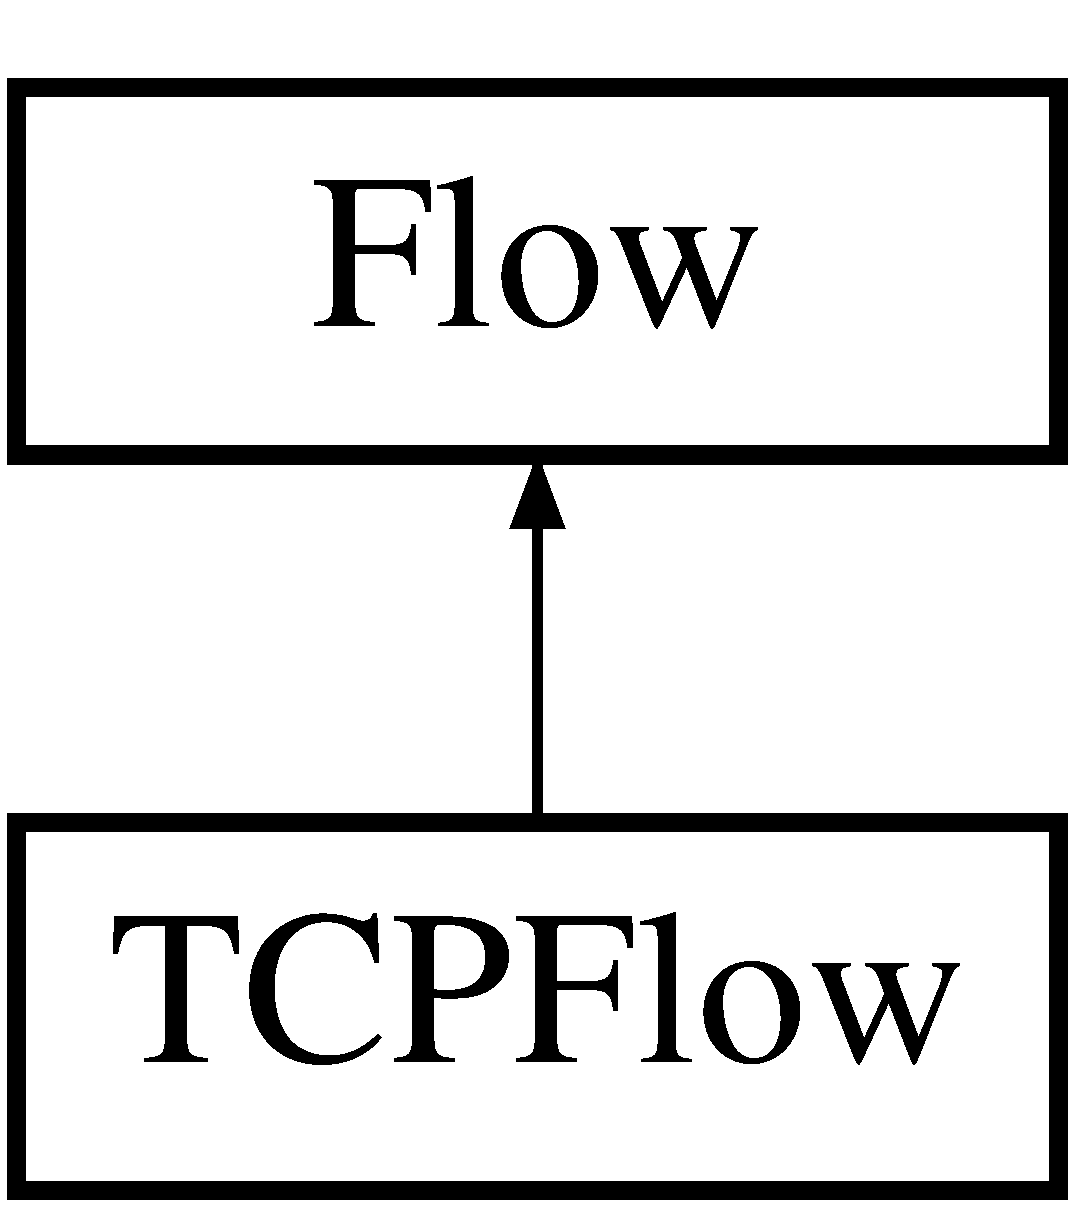
\includegraphics[height=2.000000cm]{class_t_c_p_flow}
\end{center}
\end{figure}
\subsection*{Public Member Functions}
\begin{DoxyCompactItemize}
\item 
\hyperlink{class_t_c_p_flow_a7fe59ac4b0710567478252f8d4ad9bb1}{T\+C\+P\+Flow} (std\+::string)
\item 
virtual \hyperlink{class_t_c_p_flow_a365f33092bd2f25a149f77da0d29ad29}{$\sim$\+T\+C\+P\+Flow} ()
\item 
bool \hyperlink{class_t_c_p_flow_a3ff0dd52eb3f3660dcb092d47da1b2f5}{handle\+Packet} (Crafter\+::\+Packet $\ast$)
\item 
uint32\+\_\+t \hyperlink{class_t_c_p_flow_a85ad192ed9d9f981ba87f6b2f79edf2a}{update\+Seq\+Number} (uint32\+\_\+t)
\item 
uint32\+\_\+t \hyperlink{class_t_c_p_flow_a4fe05bb98dfa337784489cc669a79ea2}{update\+Ack\+Number} (uint32\+\_\+t)
\item 
uint32\+\_\+t \hyperlink{class_t_c_p_flow_a1b42d5a597eb1d337f217a0974f48ffe}{get\+Balance} ()
\end{DoxyCompactItemize}
\subsection*{Static Public Member Functions}
\begin{DoxyCompactItemize}
\item 
static void \hyperlink{class_t_c_p_flow_acebd32b83a41150d51c1fb0bd4d0dacf}{update\+Key} (std\+::string \&key\+\_\+s, std\+::string \&key\+\_\+d, Crafter\+::\+IP $\ast$packet)
\end{DoxyCompactItemize}
\subsection*{Additional Inherited Members}


\subsection{Detailed Description}


Definition at line 32 of file T\+C\+P\+Flow.\+h.



\subsection{Constructor \& Destructor Documentation}
\index{T\+C\+P\+Flow@{T\+C\+P\+Flow}!T\+C\+P\+Flow@{T\+C\+P\+Flow}}
\index{T\+C\+P\+Flow@{T\+C\+P\+Flow}!T\+C\+P\+Flow@{T\+C\+P\+Flow}}
\subsubsection[{\texorpdfstring{T\+C\+P\+Flow(std\+::string)}{TCPFlow(std::string)}}]{\setlength{\rightskip}{0pt plus 5cm}T\+C\+P\+Flow\+::\+T\+C\+P\+Flow (
\begin{DoxyParamCaption}
\item[{std\+::string}]{key}
\end{DoxyParamCaption}
)}\hypertarget{class_t_c_p_flow_a7fe59ac4b0710567478252f8d4ad9bb1}{}\label{class_t_c_p_flow_a7fe59ac4b0710567478252f8d4ad9bb1}
Creates an instance from the key provided. 
\begin{DoxyParams}{Parameters}
{\em std\+::string} & key identifying this flow. \\
\hline
\end{DoxyParams}


Definition at line 29 of file T\+C\+P\+Flow.\+cpp.

\index{T\+C\+P\+Flow@{T\+C\+P\+Flow}!````~T\+C\+P\+Flow@{$\sim$\+T\+C\+P\+Flow}}
\index{````~T\+C\+P\+Flow@{$\sim$\+T\+C\+P\+Flow}!T\+C\+P\+Flow@{T\+C\+P\+Flow}}
\subsubsection[{\texorpdfstring{$\sim$\+T\+C\+P\+Flow()}{~TCPFlow()}}]{\setlength{\rightskip}{0pt plus 5cm}T\+C\+P\+Flow\+::$\sim$\+T\+C\+P\+Flow (
\begin{DoxyParamCaption}
{}
\end{DoxyParamCaption}
)\hspace{0.3cm}{\ttfamily [virtual]}}\hypertarget{class_t_c_p_flow_a365f33092bd2f25a149f77da0d29ad29}{}\label{class_t_c_p_flow_a365f33092bd2f25a149f77da0d29ad29}


Definition at line 34 of file T\+C\+P\+Flow.\+cpp.



\subsection{Member Function Documentation}
\index{T\+C\+P\+Flow@{T\+C\+P\+Flow}!get\+Balance@{get\+Balance}}
\index{get\+Balance@{get\+Balance}!T\+C\+P\+Flow@{T\+C\+P\+Flow}}
\subsubsection[{\texorpdfstring{get\+Balance()}{getBalance()}}]{\setlength{\rightskip}{0pt plus 5cm}uint32\+\_\+t T\+C\+P\+Flow\+::get\+Balance (
\begin{DoxyParamCaption}
{}
\end{DoxyParamCaption}
)\hspace{0.3cm}{\ttfamily [inline]}}\hypertarget{class_t_c_p_flow_a1b42d5a597eb1d337f217a0974f48ffe}{}\label{class_t_c_p_flow_a1b42d5a597eb1d337f217a0974f48ffe}
Returns the current balance \begin{DoxyReturn}{Returns}
uint32\+\_\+t 
\end{DoxyReturn}


Definition at line 78 of file T\+C\+P\+Flow.\+h.

\index{T\+C\+P\+Flow@{T\+C\+P\+Flow}!handle\+Packet@{handle\+Packet}}
\index{handle\+Packet@{handle\+Packet}!T\+C\+P\+Flow@{T\+C\+P\+Flow}}
\subsubsection[{\texorpdfstring{handle\+Packet(\+Crafter\+::\+Packet $\ast$)}{handlePacket(Crafter::Packet *)}}]{\setlength{\rightskip}{0pt plus 5cm}bool T\+C\+P\+Flow\+::handle\+Packet (
\begin{DoxyParamCaption}
\item[{Crafter\+::\+Packet $\ast$}]{packet}
\end{DoxyParamCaption}
)\hspace{0.3cm}{\ttfamily [virtual]}}\hypertarget{class_t_c_p_flow_a3ff0dd52eb3f3660dcb092d47da1b2f5}{}\label{class_t_c_p_flow_a3ff0dd52eb3f3660dcb092d47da1b2f5}
If a packet matches it with a pattern it will update it. Handles seq and ack numbers to make everything traspartent. Once modify it will update further packets inside this connection. Use its brother to keep everything consistent. 
\begin{DoxyParams}{Parameters}
{\em Crafter\+::\+Packet$\ast$} & to be handled. This object may be modified. \\
\hline
\end{DoxyParams}
\begin{DoxyReturn}{Returns}
bool. True if packet was modified. 
\end{DoxyReturn}
T\+CP Will be placed always inside IP. 

Implements \hyperlink{class_flow_aabcb243e3a9c04c1eb9b1090a3520544}{Flow}.



Definition at line 43 of file T\+C\+P\+Flow.\+cpp.

\index{T\+C\+P\+Flow@{T\+C\+P\+Flow}!update\+Ack\+Number@{update\+Ack\+Number}}
\index{update\+Ack\+Number@{update\+Ack\+Number}!T\+C\+P\+Flow@{T\+C\+P\+Flow}}
\subsubsection[{\texorpdfstring{update\+Ack\+Number(uint32\+\_\+t)}{updateAckNumber(uint32_t)}}]{\setlength{\rightskip}{0pt plus 5cm}uint32\+\_\+t T\+C\+P\+Flow\+::update\+Ack\+Number (
\begin{DoxyParamCaption}
\item[{uint32\+\_\+t}]{current\+\_\+ack}
\end{DoxyParamCaption}
)}\hypertarget{class_t_c_p_flow_a4fe05bb98dfa337784489cc669a79ea2}{}\label{class_t_c_p_flow_a4fe05bb98dfa337784489cc669a79ea2}
Updates A\+CK number 
\begin{DoxyParams}{Parameters}
{\em uint32\+\_\+t} & current ack number \\
\hline
\end{DoxyParams}
\begin{DoxyReturn}{Returns}
ack number considering modifications 
\end{DoxyReturn}


Definition at line 40 of file T\+C\+P\+Flow.\+cpp.

\index{T\+C\+P\+Flow@{T\+C\+P\+Flow}!update\+Key@{update\+Key}}
\index{update\+Key@{update\+Key}!T\+C\+P\+Flow@{T\+C\+P\+Flow}}
\subsubsection[{\texorpdfstring{update\+Key(std\+::string \&key\+\_\+s, std\+::string \&key\+\_\+d, Crafter\+::\+I\+P $\ast$packet)}{updateKey(std::string &key_s, std::string &key_d, Crafter::IP *packet)}}]{\setlength{\rightskip}{0pt plus 5cm}void T\+C\+P\+Flow\+::update\+Key (
\begin{DoxyParamCaption}
\item[{std\+::string \&}]{key\+\_\+s, }
\item[{std\+::string \&}]{key\+\_\+d, }
\item[{Crafter\+::\+IP $\ast$}]{packet}
\end{DoxyParamCaption}
)\hspace{0.3cm}{\ttfamily [static]}}\hypertarget{class_t_c_p_flow_acebd32b83a41150d51c1fb0bd4d0dacf}{}\label{class_t_c_p_flow_acebd32b83a41150d51c1fb0bd4d0dacf}
Class representing a T\+CP \hyperlink{class_flow}{Flow} of information. It considers balance to update seq and ack numbers. Generates keys considering first byte pair \mbox{[}0,1\mbox{]} as sport and the second one \mbox{[}2,3\mbox{]} as dport. Updates content of strings given as parameter. 
\begin{DoxyParams}{Parameters}
{\em std\+::string} & \& key source direct multiplexing key \\
\hline
{\em std\+::string} & \& key destination opposite multiplexing key \\
\hline
{\em Crafter\+::\+I\+P$\ast$} & packet packet to take data from \\
\hline
\end{DoxyParams}


Definition at line 89 of file T\+C\+P\+Flow.\+cpp.

\index{T\+C\+P\+Flow@{T\+C\+P\+Flow}!update\+Seq\+Number@{update\+Seq\+Number}}
\index{update\+Seq\+Number@{update\+Seq\+Number}!T\+C\+P\+Flow@{T\+C\+P\+Flow}}
\subsubsection[{\texorpdfstring{update\+Seq\+Number(uint32\+\_\+t)}{updateSeqNumber(uint32_t)}}]{\setlength{\rightskip}{0pt plus 5cm}uint32\+\_\+t T\+C\+P\+Flow\+::update\+Seq\+Number (
\begin{DoxyParamCaption}
\item[{uint32\+\_\+t}]{current\+\_\+seq}
\end{DoxyParamCaption}
)}\hypertarget{class_t_c_p_flow_a85ad192ed9d9f981ba87f6b2f79edf2a}{}\label{class_t_c_p_flow_a85ad192ed9d9f981ba87f6b2f79edf2a}
Updates Seq number 
\begin{DoxyParams}{Parameters}
{\em uint32\+\_\+t} & current sequence number \\
\hline
\end{DoxyParams}
\begin{DoxyReturn}{Returns}
sequence number considering modifications 
\end{DoxyReturn}


Definition at line 37 of file T\+C\+P\+Flow.\+cpp.



The documentation for this class was generated from the following files\+:\begin{DoxyCompactItemize}
\item 
/home/xshell/git/\+Reht\+Se/include/flows/\hyperlink{_t_c_p_flow_8h}{T\+C\+P\+Flow.\+h}\item 
/home/xshell/git/\+Reht\+Se/src/flows/\hyperlink{_t_c_p_flow_8cpp}{T\+C\+P\+Flow.\+cpp}\end{DoxyCompactItemize}

\hypertarget{class_user_interface}{}\section{User\+Interface Class Reference}
\label{class_user_interface}\index{User\+Interface@{User\+Interface}}


{\ttfamily \#include $<$User\+Interface.\+h$>$}

\subsection*{Public Member Functions}
\begin{DoxyCompactItemize}
\item 
\hyperlink{class_user_interface_ae6fb70370701b3bd6120e923df9705b0}{User\+Interface} ()
\item 
virtual \hyperlink{class_user_interface_ae588b2ff1711a016dd4c6fc5002c0841}{$\sim$\+User\+Interface} ()
\item 
void \hyperlink{class_user_interface_a6d8d6d6b6900823be51259efba78b400}{run} ()
\item 
void \hyperlink{class_user_interface_a79350878c72585ae34e4321613ed2c1a}{start} ()
\item 
void \hyperlink{class_user_interface_aed9ff11dad1ecd1611498771b63bc47d}{quit} ()
\item 
void \hyperlink{class_user_interface_a66e0842cd0c15c03162bdbb4b1a8583b}{init\+\_\+logging} (boost\+::log\+::trivial\+::severity\+\_\+level)
\end{DoxyCompactItemize}
\subsection*{Static Public Attributes}
\begin{DoxyCompactItemize}
\item 
static const char \hyperlink{class_user_interface_ae4736080db86b9df78359826bd993cc5}{O\+P\+\_\+\+C\+O\+D\+E\+\_\+\+S\+H\+OW} =\textquotesingle{}s\textquotesingle{}
\item 
static const char \hyperlink{class_user_interface_a20eef406b46e1b32db660b50cf30e796}{O\+P\+\_\+\+C\+O\+D\+E\+\_\+\+Q\+U\+IT} =\textquotesingle{}q\textquotesingle{}
\end{DoxyCompactItemize}


\subsection{Detailed Description}


Definition at line 47 of file User\+Interface.\+h.



\subsection{Constructor \& Destructor Documentation}
\index{User\+Interface@{User\+Interface}!User\+Interface@{User\+Interface}}
\index{User\+Interface@{User\+Interface}!User\+Interface@{User\+Interface}}
\subsubsection[{\texorpdfstring{User\+Interface()}{UserInterface()}}]{\setlength{\rightskip}{0pt plus 5cm}User\+Interface\+::\+User\+Interface (
\begin{DoxyParamCaption}
{}
\end{DoxyParamCaption}
)}\hypertarget{class_user_interface_ae6fb70370701b3bd6120e923df9705b0}{}\label{class_user_interface_ae6fb70370701b3bd6120e923df9705b0}
\hyperlink{class_user_interface_ae6fb70370701b3bd6120e923df9705b0}{User\+Interface()} Not much to say, initializes logger. In the future it will configure filename instead of using hardcoded config.\+json. 

Definition at line 28 of file User\+Interface.\+cpp.

\index{User\+Interface@{User\+Interface}!````~User\+Interface@{$\sim$\+User\+Interface}}
\index{````~User\+Interface@{$\sim$\+User\+Interface}!User\+Interface@{User\+Interface}}
\subsubsection[{\texorpdfstring{$\sim$\+User\+Interface()}{~UserInterface()}}]{\setlength{\rightskip}{0pt plus 5cm}User\+Interface\+::$\sim$\+User\+Interface (
\begin{DoxyParamCaption}
{}
\end{DoxyParamCaption}
)\hspace{0.3cm}{\ttfamily [virtual]}}\hypertarget{class_user_interface_ae588b2ff1711a016dd4c6fc5002c0841}{}\label{class_user_interface_ae588b2ff1711a016dd4c6fc5002c0841}


Definition at line 32 of file User\+Interface.\+cpp.



\subsection{Member Function Documentation}
\index{User\+Interface@{User\+Interface}!init\+\_\+logging@{init\+\_\+logging}}
\index{init\+\_\+logging@{init\+\_\+logging}!User\+Interface@{User\+Interface}}
\subsubsection[{\texorpdfstring{init\+\_\+logging(boost\+::log\+::trivial\+::severity\+\_\+level)}{init_logging(boost::log::trivial::severity_level)}}]{\setlength{\rightskip}{0pt plus 5cm}void User\+Interface\+::init\+\_\+logging (
\begin{DoxyParamCaption}
\item[{boost\+::log\+::trivial\+::severity\+\_\+level}]{severity}
\end{DoxyParamCaption}
)}\hypertarget{class_user_interface_a66e0842cd0c15c03162bdbb4b1a8583b}{}\label{class_user_interface_a66e0842cd0c15c03162bdbb4b1a8583b}
Initializes logging without file, just to S\+T\+D\+O\+UT. 
\begin{DoxyParams}{Parameters}
{\em boost\+::log\+::trivial\+::severity\+\_\+level} & \\
\hline
\end{DoxyParams}


Definition at line 35 of file User\+Interface.\+cpp.

\index{User\+Interface@{User\+Interface}!quit@{quit}}
\index{quit@{quit}!User\+Interface@{User\+Interface}}
\subsubsection[{\texorpdfstring{quit()}{quit()}}]{\setlength{\rightskip}{0pt plus 5cm}void User\+Interface\+::quit (
\begin{DoxyParamCaption}
{}
\end{DoxyParamCaption}
)}\hypertarget{class_user_interface_aed9ff11dad1ecd1611498771b63bc47d}{}\label{class_user_interface_aed9ff11dad1ecd1611498771b63bc47d}
\hyperlink{class_user_interface_aed9ff11dad1ecd1611498771b63bc47d}{quit()} Releases all and exits 

Definition at line 48 of file User\+Interface.\+cpp.

\index{User\+Interface@{User\+Interface}!run@{run}}
\index{run@{run}!User\+Interface@{User\+Interface}}
\subsubsection[{\texorpdfstring{run()}{run()}}]{\setlength{\rightskip}{0pt plus 5cm}void User\+Interface\+::run (
\begin{DoxyParamCaption}
{}
\end{DoxyParamCaption}
)}\hypertarget{class_user_interface_a6d8d6d6b6900823be51259efba78b400}{}\label{class_user_interface_a6d8d6d6b6900823be51259efba78b400}
\hyperlink{class_user_interface_a6d8d6d6b6900823be51259efba78b400}{run()} Parses config.\+json. Instantiates \hyperlink{class_scanner}{Scanner} and add as patterns as defined in the file. 

Definition at line 54 of file User\+Interface.\+cpp.

\index{User\+Interface@{User\+Interface}!start@{start}}
\index{start@{start}!User\+Interface@{User\+Interface}}
\subsubsection[{\texorpdfstring{start()}{start()}}]{\setlength{\rightskip}{0pt plus 5cm}void User\+Interface\+::start (
\begin{DoxyParamCaption}
{}
\end{DoxyParamCaption}
)}\hypertarget{class_user_interface_a79350878c72585ae34e4321613ed2c1a}{}\label{class_user_interface_a79350878c72585ae34e4321613ed2c1a}
\hyperlink{class_user_interface_a79350878c72585ae34e4321613ed2c1a}{start()} Initializes Crafter. In the future any necessary previous operations will be performed here. 

Definition at line 44 of file User\+Interface.\+cpp.



\subsection{Member Data Documentation}
\index{User\+Interface@{User\+Interface}!O\+P\+\_\+\+C\+O\+D\+E\+\_\+\+Q\+U\+IT@{O\+P\+\_\+\+C\+O\+D\+E\+\_\+\+Q\+U\+IT}}
\index{O\+P\+\_\+\+C\+O\+D\+E\+\_\+\+Q\+U\+IT@{O\+P\+\_\+\+C\+O\+D\+E\+\_\+\+Q\+U\+IT}!User\+Interface@{User\+Interface}}
\subsubsection[{\texorpdfstring{O\+P\+\_\+\+C\+O\+D\+E\+\_\+\+Q\+U\+IT}{OP_CODE_QUIT}}]{\setlength{\rightskip}{0pt plus 5cm}const char User\+Interface\+::\+O\+P\+\_\+\+C\+O\+D\+E\+\_\+\+Q\+U\+IT =\textquotesingle{}q\textquotesingle{}\hspace{0.3cm}{\ttfamily [static]}}\hypertarget{class_user_interface_a20eef406b46e1b32db660b50cf30e796}{}\label{class_user_interface_a20eef406b46e1b32db660b50cf30e796}


Definition at line 53 of file User\+Interface.\+h.

\index{User\+Interface@{User\+Interface}!O\+P\+\_\+\+C\+O\+D\+E\+\_\+\+S\+H\+OW@{O\+P\+\_\+\+C\+O\+D\+E\+\_\+\+S\+H\+OW}}
\index{O\+P\+\_\+\+C\+O\+D\+E\+\_\+\+S\+H\+OW@{O\+P\+\_\+\+C\+O\+D\+E\+\_\+\+S\+H\+OW}!User\+Interface@{User\+Interface}}
\subsubsection[{\texorpdfstring{O\+P\+\_\+\+C\+O\+D\+E\+\_\+\+S\+H\+OW}{OP_CODE_SHOW}}]{\setlength{\rightskip}{0pt plus 5cm}const char User\+Interface\+::\+O\+P\+\_\+\+C\+O\+D\+E\+\_\+\+S\+H\+OW =\textquotesingle{}s\textquotesingle{}\hspace{0.3cm}{\ttfamily [static]}}\hypertarget{class_user_interface_ae4736080db86b9df78359826bd993cc5}{}\label{class_user_interface_ae4736080db86b9df78359826bd993cc5}
Class designed to interact with user. 

Definition at line 52 of file User\+Interface.\+h.



The documentation for this class was generated from the following files\+:\begin{DoxyCompactItemize}
\item 
/home/xshell/git/\+Reht\+Se/include/\hyperlink{_user_interface_8h}{User\+Interface.\+h}\item 
/home/xshell/git/\+Reht\+Se/src/\hyperlink{_user_interface_8cpp}{User\+Interface.\+cpp}\end{DoxyCompactItemize}

\chapter{File Documentation}
\hypertarget{_flow_8d}{}\section{/home/xshell/git/\+Reht\+Se/\+Debug/src/flows/\+Flow.d File Reference}
\label{_flow_8d}\index{/home/xshell/git/\+Reht\+Se/\+Debug/src/flows/\+Flow.\+d@{/home/xshell/git/\+Reht\+Se/\+Debug/src/flows/\+Flow.\+d}}

\hypertarget{_flow_tracker_8d}{}\section{/home/xshell/git/\+Reht\+Se/\+Debug/src/flows/\+Flow\+Tracker.d File Reference}
\label{_flow_tracker_8d}\index{/home/xshell/git/\+Reht\+Se/\+Debug/src/flows/\+Flow\+Tracker.\+d@{/home/xshell/git/\+Reht\+Se/\+Debug/src/flows/\+Flow\+Tracker.\+d}}

\hypertarget{_generic_flow_8d}{}\section{/home/xshell/git/\+Reht\+Se/\+Debug/src/flows/\+Generic\+Flow.d File Reference}
\label{_generic_flow_8d}\index{/home/xshell/git/\+Reht\+Se/\+Debug/src/flows/\+Generic\+Flow.\+d@{/home/xshell/git/\+Reht\+Se/\+Debug/src/flows/\+Generic\+Flow.\+d}}

\hypertarget{_peer_8d}{}\section{/home/xshell/git/\+Reht\+Se/\+Debug/src/flows/\+Peer.d File Reference}
\label{_peer_8d}\index{/home/xshell/git/\+Reht\+Se/\+Debug/src/flows/\+Peer.\+d@{/home/xshell/git/\+Reht\+Se/\+Debug/src/flows/\+Peer.\+d}}

\hypertarget{_t_c_p_flow_8d}{}\section{/home/xshell/git/\+Reht\+Se/\+Debug/src/flows/\+T\+C\+P\+Flow.d File Reference}
\label{_t_c_p_flow_8d}\index{/home/xshell/git/\+Reht\+Se/\+Debug/src/flows/\+T\+C\+P\+Flow.\+d@{/home/xshell/git/\+Reht\+Se/\+Debug/src/flows/\+T\+C\+P\+Flow.\+d}}

\hypertarget{main_8d}{}\section{/home/xshell/git/\+Reht\+Se/\+Debug/src/main.d File Reference}
\label{main_8d}\index{/home/xshell/git/\+Reht\+Se/\+Debug/src/main.\+d@{/home/xshell/git/\+Reht\+Se/\+Debug/src/main.\+d}}

\hypertarget{misc_8d}{}\section{/home/xshell/git/\+Reht\+Se/\+Debug/src/misc.d File Reference}
\label{misc_8d}\index{/home/xshell/git/\+Reht\+Se/\+Debug/src/misc.\+d@{/home/xshell/git/\+Reht\+Se/\+Debug/src/misc.\+d}}

\hypertarget{_n_f_queue_8d}{}\section{/home/xshell/git/\+Reht\+Se/\+Debug/src/\+N\+F\+Queue.d File Reference}
\label{_n_f_queue_8d}\index{/home/xshell/git/\+Reht\+Se/\+Debug/src/\+N\+F\+Queue.\+d@{/home/xshell/git/\+Reht\+Se/\+Debug/src/\+N\+F\+Queue.\+d}}

\hypertarget{_pattern_8d}{}\section{/home/xshell/git/\+Reht\+Se/\+Debug/src/pattern/\+Pattern.d File Reference}
\label{_pattern_8d}\index{/home/xshell/git/\+Reht\+Se/\+Debug/src/pattern/\+Pattern.\+d@{/home/xshell/git/\+Reht\+Se/\+Debug/src/pattern/\+Pattern.\+d}}

\hypertarget{_scanner_8d}{}\section{/home/xshell/git/\+Reht\+Se/\+Debug/src/pattern/\+Scanner.d File Reference}
\label{_scanner_8d}\index{/home/xshell/git/\+Reht\+Se/\+Debug/src/pattern/\+Scanner.\+d@{/home/xshell/git/\+Reht\+Se/\+Debug/src/pattern/\+Scanner.\+d}}

\hypertarget{_u_i_8d}{}\section{/home/xshell/git/\+Reht\+Se/\+Debug/src/\+UI.d File Reference}
\label{_u_i_8d}\index{/home/xshell/git/\+Reht\+Se/\+Debug/src/\+U\+I.\+d@{/home/xshell/git/\+Reht\+Se/\+Debug/src/\+U\+I.\+d}}

\hypertarget{_user_interface_8d}{}\section{/home/xshell/git/\+Reht\+Se/\+Debug/src/\+User\+Interface.d File Reference}
\label{_user_interface_8d}\index{/home/xshell/git/\+Reht\+Se/\+Debug/src/\+User\+Interface.\+d@{/home/xshell/git/\+Reht\+Se/\+Debug/src/\+User\+Interface.\+d}}

\hypertarget{err_8h}{}\section{/home/xshell/git/\+Reht\+Se/include/err.h File Reference}
\label{err_8h}\index{/home/xshell/git/\+Reht\+Se/include/err.\+h@{/home/xshell/git/\+Reht\+Se/include/err.\+h}}
\subsection*{Macros}
\begin{DoxyCompactItemize}
\item 
\#define \hyperlink{err_8h_a9df34cfb382d46df54c3e65d937c2971}{\+\_\+\+E\+RR}
\end{DoxyCompactItemize}


\subsection{Macro Definition Documentation}
\index{err.\+h@{err.\+h}!\+\_\+\+E\+RR@{\+\_\+\+E\+RR}}
\index{\+\_\+\+E\+RR@{\+\_\+\+E\+RR}!err.\+h@{err.\+h}}
\subsubsection[{\texorpdfstring{\+\_\+\+E\+RR}{_ERR}}]{\setlength{\rightskip}{0pt plus 5cm}\#define \+\_\+\+E\+RR}\hypertarget{err_8h_a9df34cfb382d46df54c3e65d937c2971}{}\label{err_8h_a9df34cfb382d46df54c3e65d937c2971}


Definition at line 28 of file err.\+h.


\hypertarget{_flow_8h}{}\section{/home/xshell/git/\+Reht\+Se/include/flows/\+Flow.h File Reference}
\label{_flow_8h}\index{/home/xshell/git/\+Reht\+Se/include/flows/\+Flow.\+h@{/home/xshell/git/\+Reht\+Se/include/flows/\+Flow.\+h}}
{\ttfamily \#include $<$arpa/inet.\+h$>$}\\*
{\ttfamily \#include $<$crafter.\+h$>$}\\*
{\ttfamily \#include $<$boost/log/core.\+hpp$>$}\\*
{\ttfamily \#include $<$boost/log/trivial.\+hpp$>$}\\*
{\ttfamily \#include $<$boost/log/expressions.\+hpp$>$}\\*
{\ttfamily \#include $<$misc.\+h$>$}\\*
{\ttfamily \#include $<$boost/regex.\+hpp$>$}\\*
\subsection*{Classes}
\begin{DoxyCompactItemize}
\item 
class \hyperlink{class_flow}{Flow}
\end{DoxyCompactItemize}

\hypertarget{_flow_tracker_8h}{}\section{/home/xshell/git/\+Reht\+Se/include/flows/\+Flow\+Tracker.h File Reference}
\label{_flow_tracker_8h}\index{/home/xshell/git/\+Reht\+Se/include/flows/\+Flow\+Tracker.\+h@{/home/xshell/git/\+Reht\+Se/include/flows/\+Flow\+Tracker.\+h}}
{\ttfamily \#include $<$crafter.\+h$>$}\\*
{\ttfamily \#include $<$radix\+\_\+tree.\+hpp$>$}\\*
{\ttfamily \#include $<$flows/\+Flow.\+h$>$}\\*
{\ttfamily \#include $<$boost/log/core.\+hpp$>$}\\*
{\ttfamily \#include $<$boost/log/trivial.\+hpp$>$}\\*
{\ttfamily \#include $<$boost/log/expressions.\+hpp$>$}\\*
{\ttfamily \#include $<$misc.\+h$>$}\\*
\subsection*{Classes}
\begin{DoxyCompactItemize}
\item 
class \hyperlink{class_flow_tracker}{Flow\+Tracker}
\end{DoxyCompactItemize}

\hypertarget{_generic_flow_8h}{}\section{/home/xshell/git/\+Reht\+Se/include/flows/\+Generic\+Flow.h File Reference}
\label{_generic_flow_8h}\index{/home/xshell/git/\+Reht\+Se/include/flows/\+Generic\+Flow.\+h@{/home/xshell/git/\+Reht\+Se/include/flows/\+Generic\+Flow.\+h}}
{\ttfamily \#include $<$flows/\+Flow.\+h$>$}\\*
{\ttfamily \#include $<$pattern/\+Scanner.\+h$>$}\\*
{\ttfamily \#include $<$pattern/\+Pattern.\+h$>$}\\*
\subsection*{Classes}
\begin{DoxyCompactItemize}
\item 
class \hyperlink{class_generic_flow}{Generic\+Flow}
\end{DoxyCompactItemize}

\hypertarget{_t_c_p_flow_8h}{}\section{/home/xshell/git/\+Reht\+Se/include/flows/\+T\+C\+P\+Flow.h File Reference}
\label{_t_c_p_flow_8h}\index{/home/xshell/git/\+Reht\+Se/include/flows/\+T\+C\+P\+Flow.\+h@{/home/xshell/git/\+Reht\+Se/include/flows/\+T\+C\+P\+Flow.\+h}}
{\ttfamily \#include $<$flows/\+Flow.\+h$>$}\\*
{\ttfamily \#include $<$pattern/\+Scanner.\+h$>$}\\*
\subsection*{Classes}
\begin{DoxyCompactItemize}
\item 
class \hyperlink{class_t_c_p_flow}{T\+C\+P\+Flow}
\end{DoxyCompactItemize}

\hypertarget{misc_8h}{}\section{/home/xshell/git/\+Reht\+Se/include/misc.h File Reference}
\label{misc_8h}\index{/home/xshell/git/\+Reht\+Se/include/misc.\+h@{/home/xshell/git/\+Reht\+Se/include/misc.\+h}}
{\ttfamily \#include $<$boost/asio.\+hpp$>$}\\*
{\ttfamily \#include $<$boost/bind.\+hpp$>$}\\*
{\ttfamily \#include $<$boost/format.\+hpp$>$}\\*
{\ttfamily \#include $<$iostream$>$}\\*
{\ttfamily \#include $<$set$>$}\\*
{\ttfamily \#include $<$map$>$}\\*
{\ttfamily \#include $<$string$>$}\\*
{\ttfamily \#include $<$net/ethernet.\+h$>$}\\*
{\ttfamily \#include $<$net/if\+\_\+arp.\+h$>$}\\*
{\ttfamily \#include $<$netinet/if\+\_\+ether.\+h$>$}\\*
\subsection*{Macros}
\begin{DoxyCompactItemize}
\item 
\#define \hyperlink{misc_8h_adc9fcc1ff8224752ddf74b9e62adb44f}{\+\_\+\+M\+I\+SC}
\end{DoxyCompactItemize}
\subsection*{Typedefs}
\begin{DoxyCompactItemize}
\item 
typedef boost\+::asio\+::generic\+::raw\+\_\+protocol \hyperlink{misc_8h_a588ff42749a655a5c2facfe521dee292}{raw\+\_\+protocol\+\_\+t}
\item 
typedef boost\+::asio\+::generic\+::basic\+\_\+endpoint$<$ \hyperlink{misc_8h_a588ff42749a655a5c2facfe521dee292}{raw\+\_\+protocol\+\_\+t} $>$ \hyperlink{misc_8h_a8ecd3c4f6eb9ecceaef7d16699844e97}{raw\+\_\+endpoint\+\_\+t}
\end{DoxyCompactItemize}
\subsection*{Functions}
\begin{DoxyCompactItemize}
\item 
std\+::string \hyperlink{misc_8h_aee1c18572400116715202d5df122941d}{hexa\+\_\+print} (const unsigned char $\ast$array, int lenght)
\item 
std\+::string \hyperlink{misc_8h_aa7e729572a36d0773255024fbc1076c9}{hexa\+\_\+print} (const char $\ast$array, int lenght)
\item 
bool \hyperlink{misc_8h_af14f80c6b321f2805138e03b832c9091}{match\+\_\+regex} (std\+::string target, boost\+::regex regex)
\end{DoxyCompactItemize}
\subsection*{Variables}
\begin{DoxyCompactItemize}
\item 
const std\+::string \hyperlink{misc_8h_a9f3835402fa4cd5cf9e8a893dd2ad50d}{C\+O\+N\+F\+\_\+\+K\+E\+Y\+\_\+\+L\+O\+G\+L\+E\+V\+EL} =\char`\"{}debuglevel\char`\"{}
\item 
const std\+::string \hyperlink{misc_8h_a3ce1abda25fbb8efa77515b68792409c}{C\+O\+N\+F\+\_\+\+K\+E\+Y\+\_\+\+P\+A\+T\+T\+E\+R\+NS} =\char`\"{}patterns\char`\"{}
\item 
const std\+::string \hyperlink{misc_8h_abee3879c3423745f91f3889639d58709}{C\+O\+N\+F\+\_\+\+K\+E\+Y\+\_\+\+M\+A\+T\+CH} =\char`\"{}match\char`\"{}
\item 
const std\+::string \hyperlink{misc_8h_a78ae67eeac5f35df8960b4f2ec256cb8}{C\+O\+N\+F\+\_\+\+K\+E\+Y\+\_\+\+M\+O\+D\+I\+FY} =\char`\"{}modify\char`\"{}
\item 
const std\+::string \hyperlink{misc_8h_ab56c159876f6acd54ea5297d5a003c6d}{C\+O\+N\+F\+\_\+\+K\+E\+Y\+\_\+\+R\+E\+P\+L\+A\+C\+E\+M\+E\+NT} =\char`\"{}replacement\char`\"{}
\item 
const std\+::string \hyperlink{misc_8h_abf3449c5c0efb6b896555f1e3e651d21}{C\+O\+N\+F\+\_\+\+K\+E\+Y\+\_\+\+R\+E\+G\+EX} =\char`\"{}regex\char`\"{}
\item 
const std\+::string \hyperlink{misc_8h_a72f2f4f65d0b3d6110cf79a17359747e}{C\+O\+N\+F\+\_\+\+K\+E\+Y\+\_\+\+B\+PF} =\char`\"{}bpf\char`\"{}
\end{DoxyCompactItemize}


\subsection{Macro Definition Documentation}
\index{misc.\+h@{misc.\+h}!\+\_\+\+M\+I\+SC@{\+\_\+\+M\+I\+SC}}
\index{\+\_\+\+M\+I\+SC@{\+\_\+\+M\+I\+SC}!misc.\+h@{misc.\+h}}
\subsubsection[{\texorpdfstring{\+\_\+\+M\+I\+SC}{_MISC}}]{\setlength{\rightskip}{0pt plus 5cm}\#define \+\_\+\+M\+I\+SC}\hypertarget{misc_8h_adc9fcc1ff8224752ddf74b9e62adb44f}{}\label{misc_8h_adc9fcc1ff8224752ddf74b9e62adb44f}


Definition at line 28 of file misc.\+h.



\subsection{Typedef Documentation}
\index{misc.\+h@{misc.\+h}!raw\+\_\+endpoint\+\_\+t@{raw\+\_\+endpoint\+\_\+t}}
\index{raw\+\_\+endpoint\+\_\+t@{raw\+\_\+endpoint\+\_\+t}!misc.\+h@{misc.\+h}}
\subsubsection[{\texorpdfstring{raw\+\_\+endpoint\+\_\+t}{raw_endpoint_t}}]{\setlength{\rightskip}{0pt plus 5cm}typedef boost\+::asio\+::generic\+::basic\+\_\+endpoint$<${\bf raw\+\_\+protocol\+\_\+t}$>$ {\bf raw\+\_\+endpoint\+\_\+t}}\hypertarget{misc_8h_a8ecd3c4f6eb9ecceaef7d16699844e97}{}\label{misc_8h_a8ecd3c4f6eb9ecceaef7d16699844e97}


Definition at line 49 of file misc.\+h.

\index{misc.\+h@{misc.\+h}!raw\+\_\+protocol\+\_\+t@{raw\+\_\+protocol\+\_\+t}}
\index{raw\+\_\+protocol\+\_\+t@{raw\+\_\+protocol\+\_\+t}!misc.\+h@{misc.\+h}}
\subsubsection[{\texorpdfstring{raw\+\_\+protocol\+\_\+t}{raw_protocol_t}}]{\setlength{\rightskip}{0pt plus 5cm}typedef boost\+::asio\+::generic\+::raw\+\_\+protocol {\bf raw\+\_\+protocol\+\_\+t}}\hypertarget{misc_8h_a588ff42749a655a5c2facfe521dee292}{}\label{misc_8h_a588ff42749a655a5c2facfe521dee292}


Definition at line 48 of file misc.\+h.



\subsection{Function Documentation}
\index{misc.\+h@{misc.\+h}!hexa\+\_\+print@{hexa\+\_\+print}}
\index{hexa\+\_\+print@{hexa\+\_\+print}!misc.\+h@{misc.\+h}}
\subsubsection[{\texorpdfstring{hexa\+\_\+print(const unsigned char $\ast$array, int lenght)}{hexa_print(const unsigned char *array, int lenght)}}]{\setlength{\rightskip}{0pt plus 5cm}std\+::string hexa\+\_\+print (
\begin{DoxyParamCaption}
\item[{const unsigned char $\ast$}]{array, }
\item[{int}]{lenght}
\end{DoxyParamCaption}
)}\hypertarget{misc_8h_aee1c18572400116715202d5df122941d}{}\label{misc_8h_aee1c18572400116715202d5df122941d}
Formats the array to hexadecimal. 
\begin{DoxyParams}{Parameters}
{\em const} & unsigned char$\ast$ \\
\hline
{\em int} & length \\
\hline
\end{DoxyParams}
\begin{DoxyReturn}{Returns}
std\+::string containing hexadecimal representation of the array. 
\end{DoxyReturn}


Definition at line 33 of file misc.\+cpp.

\index{misc.\+h@{misc.\+h}!hexa\+\_\+print@{hexa\+\_\+print}}
\index{hexa\+\_\+print@{hexa\+\_\+print}!misc.\+h@{misc.\+h}}
\subsubsection[{\texorpdfstring{hexa\+\_\+print(const char $\ast$array, int lenght)}{hexa_print(const char *array, int lenght)}}]{\setlength{\rightskip}{0pt plus 5cm}std\+::string hexa\+\_\+print (
\begin{DoxyParamCaption}
\item[{const char $\ast$}]{array, }
\item[{int}]{lenght}
\end{DoxyParamCaption}
)}\hypertarget{misc_8h_aa7e729572a36d0773255024fbc1076c9}{}\label{misc_8h_aa7e729572a36d0773255024fbc1076c9}
Formats the array to hexadecimal. 
\begin{DoxyParams}{Parameters}
{\em const} & char$\ast$ \\
\hline
{\em int} & length \\
\hline
\end{DoxyParams}
\begin{DoxyReturn}{Returns}
std\+::string containing hexadecimal representation of the array. 
\end{DoxyReturn}


Definition at line 43 of file misc.\+cpp.

\index{misc.\+h@{misc.\+h}!match\+\_\+regex@{match\+\_\+regex}}
\index{match\+\_\+regex@{match\+\_\+regex}!misc.\+h@{misc.\+h}}
\subsubsection[{\texorpdfstring{match\+\_\+regex(std\+::string target, boost\+::regex regex)}{match_regex(std::string target, boost::regex regex)}}]{\setlength{\rightskip}{0pt plus 5cm}bool match\+\_\+regex (
\begin{DoxyParamCaption}
\item[{std\+::string}]{target, }
\item[{boost\+::regex}]{regex}
\end{DoxyParamCaption}
)}\hypertarget{misc_8h_af14f80c6b321f2805138e03b832c9091}{}\label{misc_8h_af14f80c6b321f2805138e03b832c9091}
Checks the given regex over the target and returns the result. 
\begin{DoxyParams}{Parameters}
{\em std\+::string} & target content to match against regex \\
\hline
{\em boost\+::regex} & regex regex to apply \\
\hline
\end{DoxyParams}
\begin{DoxyReturn}{Returns}
true if matches. 
\end{DoxyReturn}


Definition at line 49 of file misc.\+cpp.



\subsection{Variable Documentation}
\index{misc.\+h@{misc.\+h}!C\+O\+N\+F\+\_\+\+K\+E\+Y\+\_\+\+B\+PF@{C\+O\+N\+F\+\_\+\+K\+E\+Y\+\_\+\+B\+PF}}
\index{C\+O\+N\+F\+\_\+\+K\+E\+Y\+\_\+\+B\+PF@{C\+O\+N\+F\+\_\+\+K\+E\+Y\+\_\+\+B\+PF}!misc.\+h@{misc.\+h}}
\subsubsection[{\texorpdfstring{C\+O\+N\+F\+\_\+\+K\+E\+Y\+\_\+\+B\+PF}{CONF_KEY_BPF}}]{\setlength{\rightskip}{0pt plus 5cm}const std\+::string C\+O\+N\+F\+\_\+\+K\+E\+Y\+\_\+\+B\+PF =\char`\"{}bpf\char`\"{}}\hypertarget{misc_8h_a72f2f4f65d0b3d6110cf79a17359747e}{}\label{misc_8h_a72f2f4f65d0b3d6110cf79a17359747e}


Definition at line 47 of file misc.\+h.

\index{misc.\+h@{misc.\+h}!C\+O\+N\+F\+\_\+\+K\+E\+Y\+\_\+\+L\+O\+G\+L\+E\+V\+EL@{C\+O\+N\+F\+\_\+\+K\+E\+Y\+\_\+\+L\+O\+G\+L\+E\+V\+EL}}
\index{C\+O\+N\+F\+\_\+\+K\+E\+Y\+\_\+\+L\+O\+G\+L\+E\+V\+EL@{C\+O\+N\+F\+\_\+\+K\+E\+Y\+\_\+\+L\+O\+G\+L\+E\+V\+EL}!misc.\+h@{misc.\+h}}
\subsubsection[{\texorpdfstring{C\+O\+N\+F\+\_\+\+K\+E\+Y\+\_\+\+L\+O\+G\+L\+E\+V\+EL}{CONF_KEY_LOGLEVEL}}]{\setlength{\rightskip}{0pt plus 5cm}const std\+::string C\+O\+N\+F\+\_\+\+K\+E\+Y\+\_\+\+L\+O\+G\+L\+E\+V\+EL =\char`\"{}debuglevel\char`\"{}}\hypertarget{misc_8h_a9f3835402fa4cd5cf9e8a893dd2ad50d}{}\label{misc_8h_a9f3835402fa4cd5cf9e8a893dd2ad50d}


Definition at line 41 of file misc.\+h.

\index{misc.\+h@{misc.\+h}!C\+O\+N\+F\+\_\+\+K\+E\+Y\+\_\+\+M\+A\+T\+CH@{C\+O\+N\+F\+\_\+\+K\+E\+Y\+\_\+\+M\+A\+T\+CH}}
\index{C\+O\+N\+F\+\_\+\+K\+E\+Y\+\_\+\+M\+A\+T\+CH@{C\+O\+N\+F\+\_\+\+K\+E\+Y\+\_\+\+M\+A\+T\+CH}!misc.\+h@{misc.\+h}}
\subsubsection[{\texorpdfstring{C\+O\+N\+F\+\_\+\+K\+E\+Y\+\_\+\+M\+A\+T\+CH}{CONF_KEY_MATCH}}]{\setlength{\rightskip}{0pt plus 5cm}const std\+::string C\+O\+N\+F\+\_\+\+K\+E\+Y\+\_\+\+M\+A\+T\+CH =\char`\"{}match\char`\"{}}\hypertarget{misc_8h_abee3879c3423745f91f3889639d58709}{}\label{misc_8h_abee3879c3423745f91f3889639d58709}


Definition at line 43 of file misc.\+h.

\index{misc.\+h@{misc.\+h}!C\+O\+N\+F\+\_\+\+K\+E\+Y\+\_\+\+M\+O\+D\+I\+FY@{C\+O\+N\+F\+\_\+\+K\+E\+Y\+\_\+\+M\+O\+D\+I\+FY}}
\index{C\+O\+N\+F\+\_\+\+K\+E\+Y\+\_\+\+M\+O\+D\+I\+FY@{C\+O\+N\+F\+\_\+\+K\+E\+Y\+\_\+\+M\+O\+D\+I\+FY}!misc.\+h@{misc.\+h}}
\subsubsection[{\texorpdfstring{C\+O\+N\+F\+\_\+\+K\+E\+Y\+\_\+\+M\+O\+D\+I\+FY}{CONF_KEY_MODIFY}}]{\setlength{\rightskip}{0pt plus 5cm}const std\+::string C\+O\+N\+F\+\_\+\+K\+E\+Y\+\_\+\+M\+O\+D\+I\+FY =\char`\"{}modify\char`\"{}}\hypertarget{misc_8h_a78ae67eeac5f35df8960b4f2ec256cb8}{}\label{misc_8h_a78ae67eeac5f35df8960b4f2ec256cb8}


Definition at line 44 of file misc.\+h.

\index{misc.\+h@{misc.\+h}!C\+O\+N\+F\+\_\+\+K\+E\+Y\+\_\+\+P\+A\+T\+T\+E\+R\+NS@{C\+O\+N\+F\+\_\+\+K\+E\+Y\+\_\+\+P\+A\+T\+T\+E\+R\+NS}}
\index{C\+O\+N\+F\+\_\+\+K\+E\+Y\+\_\+\+P\+A\+T\+T\+E\+R\+NS@{C\+O\+N\+F\+\_\+\+K\+E\+Y\+\_\+\+P\+A\+T\+T\+E\+R\+NS}!misc.\+h@{misc.\+h}}
\subsubsection[{\texorpdfstring{C\+O\+N\+F\+\_\+\+K\+E\+Y\+\_\+\+P\+A\+T\+T\+E\+R\+NS}{CONF_KEY_PATTERNS}}]{\setlength{\rightskip}{0pt plus 5cm}const std\+::string C\+O\+N\+F\+\_\+\+K\+E\+Y\+\_\+\+P\+A\+T\+T\+E\+R\+NS =\char`\"{}patterns\char`\"{}}\hypertarget{misc_8h_a3ce1abda25fbb8efa77515b68792409c}{}\label{misc_8h_a3ce1abda25fbb8efa77515b68792409c}


Definition at line 42 of file misc.\+h.

\index{misc.\+h@{misc.\+h}!C\+O\+N\+F\+\_\+\+K\+E\+Y\+\_\+\+R\+E\+G\+EX@{C\+O\+N\+F\+\_\+\+K\+E\+Y\+\_\+\+R\+E\+G\+EX}}
\index{C\+O\+N\+F\+\_\+\+K\+E\+Y\+\_\+\+R\+E\+G\+EX@{C\+O\+N\+F\+\_\+\+K\+E\+Y\+\_\+\+R\+E\+G\+EX}!misc.\+h@{misc.\+h}}
\subsubsection[{\texorpdfstring{C\+O\+N\+F\+\_\+\+K\+E\+Y\+\_\+\+R\+E\+G\+EX}{CONF_KEY_REGEX}}]{\setlength{\rightskip}{0pt plus 5cm}const std\+::string C\+O\+N\+F\+\_\+\+K\+E\+Y\+\_\+\+R\+E\+G\+EX =\char`\"{}regex\char`\"{}}\hypertarget{misc_8h_abf3449c5c0efb6b896555f1e3e651d21}{}\label{misc_8h_abf3449c5c0efb6b896555f1e3e651d21}


Definition at line 46 of file misc.\+h.

\index{misc.\+h@{misc.\+h}!C\+O\+N\+F\+\_\+\+K\+E\+Y\+\_\+\+R\+E\+P\+L\+A\+C\+E\+M\+E\+NT@{C\+O\+N\+F\+\_\+\+K\+E\+Y\+\_\+\+R\+E\+P\+L\+A\+C\+E\+M\+E\+NT}}
\index{C\+O\+N\+F\+\_\+\+K\+E\+Y\+\_\+\+R\+E\+P\+L\+A\+C\+E\+M\+E\+NT@{C\+O\+N\+F\+\_\+\+K\+E\+Y\+\_\+\+R\+E\+P\+L\+A\+C\+E\+M\+E\+NT}!misc.\+h@{misc.\+h}}
\subsubsection[{\texorpdfstring{C\+O\+N\+F\+\_\+\+K\+E\+Y\+\_\+\+R\+E\+P\+L\+A\+C\+E\+M\+E\+NT}{CONF_KEY_REPLACEMENT}}]{\setlength{\rightskip}{0pt plus 5cm}const std\+::string C\+O\+N\+F\+\_\+\+K\+E\+Y\+\_\+\+R\+E\+P\+L\+A\+C\+E\+M\+E\+NT =\char`\"{}replacement\char`\"{}}\hypertarget{misc_8h_ab56c159876f6acd54ea5297d5a003c6d}{}\label{misc_8h_ab56c159876f6acd54ea5297d5a003c6d}


Definition at line 45 of file misc.\+h.


\hypertarget{_n_f_queue_8h}{}\section{/home/xshell/git/\+Reht\+Se/include/\+N\+F\+Queue.h File Reference}
\label{_n_f_queue_8h}\index{/home/xshell/git/\+Reht\+Se/include/\+N\+F\+Queue.\+h@{/home/xshell/git/\+Reht\+Se/include/\+N\+F\+Queue.\+h}}
{\ttfamily \#include $<$iostream$>$}\\*
{\ttfamily \#include $<$list$>$}\\*
{\ttfamily \#include $<$iomanip$>$}\\*
{\ttfamily \#include $<$time.\+h$>$}\\*
{\ttfamily \#include $<$cstdlib$>$}\\*
{\ttfamily \#include $<$netinet/in.\+h$>$}\\*
{\ttfamily \#include $<$linux/if\+\_\+ether.\+h$>$}\\*
{\ttfamily \#include $<$boost/log/core.\+hpp$>$}\\*
{\ttfamily \#include $<$boost/log/trivial.\+hpp$>$}\\*
{\ttfamily \#include $<$boost/log/expressions.\+hpp$>$}\\*
{\ttfamily \#include $<$misc.\+h$>$}\\*
{\ttfamily \#include $<$crafter.\+h$>$}\\*
{\ttfamily \#include $<$crafter/\+Utils/\+T\+C\+P\+Connection.\+h$>$}\\*
{\ttfamily \#include $<$flows/\+Flow\+Tracker.\+h$>$}\\*
{\ttfamily \#include $<$boost/regex.\+hpp$>$}\\*
{\ttfamily \#include $<$linux/netfilter.\+h$>$}\\*
{\ttfamily \#include $<$libnetfilter\+\_\+queue/libnetfilter\+\_\+queue.\+h$>$}\\*
{\ttfamily \#include $<$libnfnetlink/libnfnetlink.\+h$>$}\\*
{\ttfamily \#include $<$libnetfilter\+\_\+queue/libnetfilter\+\_\+queue\+\_\+ipv4.\+h$>$}\\*
{\ttfamily \#include $<$boost/asio.\+hpp$>$}\\*
\subsection*{Classes}
\begin{DoxyCompactItemize}
\item 
struct \hyperlink{structnfq__data}{nfq\+\_\+data}
\item 
class \hyperlink{class_n_f_queue}{N\+F\+Queue}
\end{DoxyCompactItemize}

\hypertarget{_pattern_8h}{}\section{/home/xshell/git/\+Reht\+Se/include/pattern/\+Pattern.h File Reference}
\label{_pattern_8h}\index{/home/xshell/git/\+Reht\+Se/include/pattern/\+Pattern.\+h@{/home/xshell/git/\+Reht\+Se/include/pattern/\+Pattern.\+h}}
{\ttfamily \#include $<$iostream$>$}\\*
{\ttfamily \#include $<$string$>$}\\*
{\ttfamily \#include $<$boost/log/core.\+hpp$>$}\\*
{\ttfamily \#include $<$boost/log/trivial.\+hpp$>$}\\*
{\ttfamily \#include $<$boost/log/expressions.\+hpp$>$}\\*
{\ttfamily \#include $<$boost/property\+\_\+tree/ptree.\+hpp$>$}\\*
{\ttfamily \#include $<$boost/regex.\+hpp$>$}\\*
{\ttfamily \#include $<$crafter.\+h$>$}\\*
{\ttfamily \#include $<$pcap.\+h$>$}\\*
{\ttfamily \#include $<$misc.\+h$>$}\\*
{\ttfamily \#include $<$err.\+h$>$}\\*
\subsection*{Classes}
\begin{DoxyCompactItemize}
\item 
class \hyperlink{class_pattern}{Pattern}
\end{DoxyCompactItemize}

\hypertarget{_scanner_8h}{}\section{/home/xshell/git/\+Reht\+Se/include/pattern/\+Scanner.h File Reference}
\label{_scanner_8h}\index{/home/xshell/git/\+Reht\+Se/include/pattern/\+Scanner.\+h@{/home/xshell/git/\+Reht\+Se/include/pattern/\+Scanner.\+h}}
{\ttfamily \#include $<$cstddef$>$}\\*
{\ttfamily \#include $<$pattern/\+Pattern.\+h$>$}\\*
\subsection*{Classes}
\begin{DoxyCompactItemize}
\item 
class \hyperlink{class_scanner}{Scanner}
\end{DoxyCompactItemize}

\hypertarget{radix__tree_8hpp}{}\section{/home/xshell/git/\+Reht\+Se/include/radix\+\_\+tree.hpp File Reference}
\label{radix__tree_8hpp}\index{/home/xshell/git/\+Reht\+Se/include/radix\+\_\+tree.\+hpp@{/home/xshell/git/\+Reht\+Se/include/radix\+\_\+tree.\+hpp}}
{\ttfamily \#include $<$cassert$>$}\\*
{\ttfamily \#include $<$string$>$}\\*
{\ttfamily \#include $<$utility$>$}\\*
{\ttfamily \#include $<$vector$>$}\\*
{\ttfamily \#include \char`\"{}radix\+\_\+tree\+\_\+it.\+hpp\char`\"{}}\\*
{\ttfamily \#include \char`\"{}radix\+\_\+tree\+\_\+node.\+hpp\char`\"{}}\\*
\subsection*{Classes}
\begin{DoxyCompactItemize}
\item 
class \hyperlink{classradix__tree}{radix\+\_\+tree$<$ K, T $>$}
\end{DoxyCompactItemize}
\subsection*{Functions}
\begin{DoxyCompactItemize}
\item 
{\footnotesize template$<$typename K $>$ }\\K \hyperlink{radix__tree_8hpp_a0da9917b249b72630281a390c624ffdf}{radix\+\_\+substr} (const K \&key, int begin, int num)
\item 
{\footnotesize template$<$$>$ }\\std\+::string \hyperlink{radix__tree_8hpp_a52e97a2393f0501d22bee9d7055ba62b}{radix\+\_\+substr$<$ std\+::string $>$} (const std\+::string \&key, int begin, int num)
\item 
{\footnotesize template$<$typename K $>$ }\\K \hyperlink{radix__tree_8hpp_a6f3470047bb909a755d9c99fcc97fab5}{radix\+\_\+join} (const K \&key1, const K \&key2)
\item 
{\footnotesize template$<$$>$ }\\std\+::string \hyperlink{radix__tree_8hpp_a78977b52504471dd8bc470f666fb83e9}{radix\+\_\+join$<$ std\+::string $>$} (const std\+::string \&key1, const std\+::string \&key2)
\item 
{\footnotesize template$<$typename K $>$ }\\int \hyperlink{radix__tree_8hpp_a970b86fa7ee4c36bb1c1895c24b9a218}{radix\+\_\+length} (const K \&key)
\item 
{\footnotesize template$<$$>$ }\\int \hyperlink{radix__tree_8hpp_a1beb7f6a3f758b93834f1fabaed3a135}{radix\+\_\+length$<$ std\+::string $>$} (const std\+::string \&key)
\end{DoxyCompactItemize}


\subsection{Function Documentation}
\index{radix\+\_\+tree.\+hpp@{radix\+\_\+tree.\+hpp}!radix\+\_\+join@{radix\+\_\+join}}
\index{radix\+\_\+join@{radix\+\_\+join}!radix\+\_\+tree.\+hpp@{radix\+\_\+tree.\+hpp}}
\subsubsection[{\texorpdfstring{radix\+\_\+join(const K \&key1, const K \&key2)}{radix_join(const K &key1, const K &key2)}}]{\setlength{\rightskip}{0pt plus 5cm}template$<$typename K $>$ K radix\+\_\+join (
\begin{DoxyParamCaption}
\item[{const K \&}]{key1, }
\item[{const K \&}]{key2}
\end{DoxyParamCaption}
)}\hypertarget{radix__tree_8hpp_a6f3470047bb909a755d9c99fcc97fab5}{}\label{radix__tree_8hpp_a6f3470047bb909a755d9c99fcc97fab5}
\index{radix\+\_\+tree.\+hpp@{radix\+\_\+tree.\+hpp}!radix\+\_\+join$<$ std\+::string $>$@{radix\+\_\+join$<$ std\+::string $>$}}
\index{radix\+\_\+join$<$ std\+::string $>$@{radix\+\_\+join$<$ std\+::string $>$}!radix\+\_\+tree.\+hpp@{radix\+\_\+tree.\+hpp}}
\subsubsection[{\texorpdfstring{radix\+\_\+join$<$ std\+::string $>$(const std\+::string \&key1, const std\+::string \&key2)}{radix_join< std::string >(const std::string &key1, const std::string &key2)}}]{\setlength{\rightskip}{0pt plus 5cm}template$<$$>$ std\+::string {\bf radix\+\_\+join}$<$ std\+::string $>$ (
\begin{DoxyParamCaption}
\item[{const std\+::string \&}]{key1, }
\item[{const std\+::string \&}]{key2}
\end{DoxyParamCaption}
)\hspace{0.3cm}{\ttfamily [inline]}}\hypertarget{radix__tree_8hpp_a78977b52504471dd8bc470f666fb83e9}{}\label{radix__tree_8hpp_a78977b52504471dd8bc470f666fb83e9}


Definition at line 25 of file radix\+\_\+tree.\+hpp.

\index{radix\+\_\+tree.\+hpp@{radix\+\_\+tree.\+hpp}!radix\+\_\+length@{radix\+\_\+length}}
\index{radix\+\_\+length@{radix\+\_\+length}!radix\+\_\+tree.\+hpp@{radix\+\_\+tree.\+hpp}}
\subsubsection[{\texorpdfstring{radix\+\_\+length(const K \&key)}{radix_length(const K &key)}}]{\setlength{\rightskip}{0pt plus 5cm}template$<$typename K $>$ int radix\+\_\+length (
\begin{DoxyParamCaption}
\item[{const K \&}]{key}
\end{DoxyParamCaption}
)}\hypertarget{radix__tree_8hpp_a970b86fa7ee4c36bb1c1895c24b9a218}{}\label{radix__tree_8hpp_a970b86fa7ee4c36bb1c1895c24b9a218}
\index{radix\+\_\+tree.\+hpp@{radix\+\_\+tree.\+hpp}!radix\+\_\+length$<$ std\+::string $>$@{radix\+\_\+length$<$ std\+::string $>$}}
\index{radix\+\_\+length$<$ std\+::string $>$@{radix\+\_\+length$<$ std\+::string $>$}!radix\+\_\+tree.\+hpp@{radix\+\_\+tree.\+hpp}}
\subsubsection[{\texorpdfstring{radix\+\_\+length$<$ std\+::string $>$(const std\+::string \&key)}{radix_length< std::string >(const std::string &key)}}]{\setlength{\rightskip}{0pt plus 5cm}template$<$$>$ int {\bf radix\+\_\+length}$<$ std\+::string $>$ (
\begin{DoxyParamCaption}
\item[{const std\+::string \&}]{key}
\end{DoxyParamCaption}
)\hspace{0.3cm}{\ttfamily [inline]}}\hypertarget{radix__tree_8hpp_a1beb7f6a3f758b93834f1fabaed3a135}{}\label{radix__tree_8hpp_a1beb7f6a3f758b93834f1fabaed3a135}


Definition at line 34 of file radix\+\_\+tree.\+hpp.

\index{radix\+\_\+tree.\+hpp@{radix\+\_\+tree.\+hpp}!radix\+\_\+substr@{radix\+\_\+substr}}
\index{radix\+\_\+substr@{radix\+\_\+substr}!radix\+\_\+tree.\+hpp@{radix\+\_\+tree.\+hpp}}
\subsubsection[{\texorpdfstring{radix\+\_\+substr(const K \&key, int begin, int num)}{radix_substr(const K &key, int begin, int num)}}]{\setlength{\rightskip}{0pt plus 5cm}template$<$typename K $>$ K radix\+\_\+substr (
\begin{DoxyParamCaption}
\item[{const K \&}]{key, }
\item[{int}]{begin, }
\item[{int}]{num}
\end{DoxyParamCaption}
)}\hypertarget{radix__tree_8hpp_a0da9917b249b72630281a390c624ffdf}{}\label{radix__tree_8hpp_a0da9917b249b72630281a390c624ffdf}
\index{radix\+\_\+tree.\+hpp@{radix\+\_\+tree.\+hpp}!radix\+\_\+substr$<$ std\+::string $>$@{radix\+\_\+substr$<$ std\+::string $>$}}
\index{radix\+\_\+substr$<$ std\+::string $>$@{radix\+\_\+substr$<$ std\+::string $>$}!radix\+\_\+tree.\+hpp@{radix\+\_\+tree.\+hpp}}
\subsubsection[{\texorpdfstring{radix\+\_\+substr$<$ std\+::string $>$(const std\+::string \&key, int begin, int num)}{radix_substr< std::string >(const std::string &key, int begin, int num)}}]{\setlength{\rightskip}{0pt plus 5cm}template$<$$>$ std\+::string {\bf radix\+\_\+substr}$<$ std\+::string $>$ (
\begin{DoxyParamCaption}
\item[{const std\+::string \&}]{key, }
\item[{int}]{begin, }
\item[{int}]{num}
\end{DoxyParamCaption}
)\hspace{0.3cm}{\ttfamily [inline]}}\hypertarget{radix__tree_8hpp_a52e97a2393f0501d22bee9d7055ba62b}{}\label{radix__tree_8hpp_a52e97a2393f0501d22bee9d7055ba62b}


Definition at line 16 of file radix\+\_\+tree.\+hpp.


\hypertarget{radix__tree__it_8hpp}{}\section{/home/xshell/git/\+Reht\+Se/include/radix\+\_\+tree\+\_\+it.hpp File Reference}
\label{radix__tree__it_8hpp}\index{/home/xshell/git/\+Reht\+Se/include/radix\+\_\+tree\+\_\+it.\+hpp@{/home/xshell/git/\+Reht\+Se/include/radix\+\_\+tree\+\_\+it.\+hpp}}
{\ttfamily \#include $<$iterator$>$}\\*
\subsection*{Classes}
\begin{DoxyCompactItemize}
\item 
class \hyperlink{classradix__tree}{radix\+\_\+tree$<$ K, T $>$}
\item 
class \hyperlink{classradix__tree__node}{radix\+\_\+tree\+\_\+node$<$ K, T $>$}
\item 
class \hyperlink{classradix__tree__it}{radix\+\_\+tree\+\_\+it$<$ K, T $>$}
\end{DoxyCompactItemize}

\hypertarget{radix__tree__node_8hpp}{}\section{/home/xshell/git/\+Reht\+Se/include/radix\+\_\+tree\+\_\+node.hpp File Reference}
\label{radix__tree__node_8hpp}\index{/home/xshell/git/\+Reht\+Se/include/radix\+\_\+tree\+\_\+node.\+hpp@{/home/xshell/git/\+Reht\+Se/include/radix\+\_\+tree\+\_\+node.\+hpp}}
{\ttfamily \#include $<$map$>$}\\*
\subsection*{Classes}
\begin{DoxyCompactItemize}
\item 
class \hyperlink{classradix__tree__node}{radix\+\_\+tree\+\_\+node$<$ K, T $>$}
\end{DoxyCompactItemize}

\hypertarget{_user_interface_8h}{}\section{/home/xshell/git/\+Reht\+Se/include/\+User\+Interface.h File Reference}
\label{_user_interface_8h}\index{/home/xshell/git/\+Reht\+Se/include/\+User\+Interface.\+h@{/home/xshell/git/\+Reht\+Se/include/\+User\+Interface.\+h}}
{\ttfamily \#include $<$iostream$>$}\\*
{\ttfamily \#include $<$cstddef$>$}\\*
{\ttfamily \#include $<$fstream$>$}\\*
{\ttfamily \#include $<$boost/asio.\+hpp$>$}\\*
{\ttfamily \#include $<$boost/log/core.\+hpp$>$}\\*
{\ttfamily \#include $<$boost/log/trivial.\+hpp$>$}\\*
{\ttfamily \#include $<$boost/log/expressions.\+hpp$>$}\\*
{\ttfamily \#include $<$boost/foreach.\+hpp$>$}\\*
{\ttfamily \#include $<$boost/property\+\_\+tree/ptree.\+hpp$>$}\\*
{\ttfamily \#include $<$boost/property\+\_\+tree/json\+\_\+parser.\+hpp$>$}\\*
{\ttfamily \#include $<$boost/asio/io\+\_\+service.\+hpp$>$}\\*
{\ttfamily \#include $<$boost/thread.\+hpp$>$}\\*
{\ttfamily \#include $<$crafter.\+h$>$}\\*
{\ttfamily \#include $<$radix\+\_\+tree.\+hpp$>$}\\*
{\ttfamily \#include $<$flows/\+Flow\+Tracker.\+h$>$}\\*
{\ttfamily \#include $<$N\+F\+Queue.\+h$>$}\\*
{\ttfamily \#include $<$pattern/\+Scanner.\+h$>$}\\*
\subsection*{Classes}
\begin{DoxyCompactItemize}
\item 
class \hyperlink{class_user_interface}{User\+Interface}
\end{DoxyCompactItemize}

\hypertarget{_r_e_a_d_m_e_8md}{}\section{/home/xshell/git/\+Reht\+Se/\+R\+E\+A\+D\+ME.md File Reference}
\label{_r_e_a_d_m_e_8md}\index{/home/xshell/git/\+Reht\+Se/\+R\+E\+A\+D\+M\+E.\+md@{/home/xshell/git/\+Reht\+Se/\+R\+E\+A\+D\+M\+E.\+md}}

\hypertarget{_flow_8cpp}{}\section{/home/xshell/git/\+Reht\+Se/src/flows/\+Flow.cpp File Reference}
\label{_flow_8cpp}\index{/home/xshell/git/\+Reht\+Se/src/flows/\+Flow.\+cpp@{/home/xshell/git/\+Reht\+Se/src/flows/\+Flow.\+cpp}}
{\ttfamily \#include $<$flows/\+Flow.\+h$>$}\\*
{\ttfamily \#include $<$flows/\+T\+C\+P\+Flow.\+h$>$}\\*
{\ttfamily \#include $<$flows/\+Generic\+Flow.\+h$>$}\\*

\hypertarget{_flow_tracker_8cpp}{}\section{/home/xshell/git/\+Reht\+Se/src/flows/\+Flow\+Tracker.cpp File Reference}
\label{_flow_tracker_8cpp}\index{/home/xshell/git/\+Reht\+Se/src/flows/\+Flow\+Tracker.\+cpp@{/home/xshell/git/\+Reht\+Se/src/flows/\+Flow\+Tracker.\+cpp}}
{\ttfamily \#include $<$flows/\+Flow\+Tracker.\+h$>$}\\*
{\ttfamily \#include $<$flows/\+T\+C\+P\+Flow.\+h$>$}\\*

\hypertarget{_generic_flow_8cpp}{}\section{/home/xshell/git/\+Reht\+Se/src/flows/\+Generic\+Flow.cpp File Reference}
\label{_generic_flow_8cpp}\index{/home/xshell/git/\+Reht\+Se/src/flows/\+Generic\+Flow.\+cpp@{/home/xshell/git/\+Reht\+Se/src/flows/\+Generic\+Flow.\+cpp}}
{\ttfamily \#include $<$flows/\+Generic\+Flow.\+h$>$}\\*

\hypertarget{_t_c_p_flow_8cpp}{}\section{/home/xshell/git/\+Reht\+Se/src/flows/\+T\+C\+P\+Flow.cpp File Reference}
\label{_t_c_p_flow_8cpp}\index{/home/xshell/git/\+Reht\+Se/src/flows/\+T\+C\+P\+Flow.\+cpp@{/home/xshell/git/\+Reht\+Se/src/flows/\+T\+C\+P\+Flow.\+cpp}}
{\ttfamily \#include $<$flows/\+T\+C\+P\+Flow.\+h$>$}\\*

\hypertarget{main_8cpp}{}\section{/home/xshell/git/\+Reht\+Se/src/main.cpp File Reference}
\label{main_8cpp}\index{/home/xshell/git/\+Reht\+Se/src/main.\+cpp@{/home/xshell/git/\+Reht\+Se/src/main.\+cpp}}
{\ttfamily \#include $<$iostream$>$}\\*
{\ttfamily \#include $<$cstdlib$>$}\\*
{\ttfamily \#include $<$boost/log/core.\+hpp$>$}\\*
{\ttfamily \#include $<$boost/log/trivial.\+hpp$>$}\\*
{\ttfamily \#include $<$boost/log/expressions.\+hpp$>$}\\*
{\ttfamily \#include $<$User\+Interface.\+h$>$}\\*
{\ttfamily \#include $<$boost/program\+\_\+options.\+hpp$>$}\\*
\subsection*{Functions}
\begin{DoxyCompactItemize}
\item 
int \hyperlink{main_8cpp_a3c04138a5bfe5d72780bb7e82a18e627}{main} (int argc, char $\ast$$\ast$argv)
\end{DoxyCompactItemize}


\subsection{Function Documentation}
\index{main.\+cpp@{main.\+cpp}!main@{main}}
\index{main@{main}!main.\+cpp@{main.\+cpp}}
\subsubsection[{\texorpdfstring{main(int argc, char $\ast$$\ast$argv)}{main(int argc, char **argv)}}]{\setlength{\rightskip}{0pt plus 5cm}int main (
\begin{DoxyParamCaption}
\item[{int}]{argc, }
\item[{char $\ast$$\ast$}]{argv}
\end{DoxyParamCaption}
)}\hypertarget{main_8cpp_a3c04138a5bfe5d72780bb7e82a18e627}{}\label{main_8cpp_a3c04138a5bfe5d72780bb7e82a18e627}


Definition at line 35 of file main.\+cpp.


\hypertarget{misc_8cpp}{}\section{/home/xshell/git/\+Reht\+Se/src/misc.cpp File Reference}
\label{misc_8cpp}\index{/home/xshell/git/\+Reht\+Se/src/misc.\+cpp@{/home/xshell/git/\+Reht\+Se/src/misc.\+cpp}}
{\ttfamily \#include $<$ostream$>$}\\*
{\ttfamily \#include $<$misc.\+h$>$}\\*
{\ttfamily \#include $<$boost/log/trivial.\+hpp$>$}\\*
{\ttfamily \#include $<$boost/format.\+hpp$>$}\\*
{\ttfamily \#include $<$boost/regex.\+hpp$>$}\\*
\subsection*{Functions}
\begin{DoxyCompactItemize}
\item 
std\+::string \hyperlink{misc_8cpp_a260dad756c8854a5fdf7fbc30093b901}{hexa\+\_\+print} (const unsigned char $\ast$array, int len)
\item 
std\+::string \hyperlink{misc_8cpp_a5910bc1c76a3a44c4e27edc35ca9bb6a}{hexa\+\_\+print} (const char $\ast$array, int len)
\item 
bool \hyperlink{misc_8cpp_af14f80c6b321f2805138e03b832c9091}{match\+\_\+regex} (std\+::string target, boost\+::regex regex)
\end{DoxyCompactItemize}


\subsection{Function Documentation}
\index{misc.\+cpp@{misc.\+cpp}!hexa\+\_\+print@{hexa\+\_\+print}}
\index{hexa\+\_\+print@{hexa\+\_\+print}!misc.\+cpp@{misc.\+cpp}}
\subsubsection[{\texorpdfstring{hexa\+\_\+print(const unsigned char $\ast$array, int len)}{hexa_print(const unsigned char *array, int len)}}]{\setlength{\rightskip}{0pt plus 5cm}std\+::string hexa\+\_\+print (
\begin{DoxyParamCaption}
\item[{const unsigned char $\ast$}]{array, }
\item[{int}]{lenght}
\end{DoxyParamCaption}
)}\hypertarget{misc_8cpp_a260dad756c8854a5fdf7fbc30093b901}{}\label{misc_8cpp_a260dad756c8854a5fdf7fbc30093b901}
Formats the array to hexadecimal. 
\begin{DoxyParams}{Parameters}
{\em const} & unsigned char$\ast$ \\
\hline
{\em int} & length \\
\hline
\end{DoxyParams}
\begin{DoxyReturn}{Returns}
std\+::string containing hexadecimal representation of the array. 
\end{DoxyReturn}


Definition at line 33 of file misc.\+cpp.

\index{misc.\+cpp@{misc.\+cpp}!hexa\+\_\+print@{hexa\+\_\+print}}
\index{hexa\+\_\+print@{hexa\+\_\+print}!misc.\+cpp@{misc.\+cpp}}
\subsubsection[{\texorpdfstring{hexa\+\_\+print(const char $\ast$array, int len)}{hexa_print(const char *array, int len)}}]{\setlength{\rightskip}{0pt plus 5cm}std\+::string hexa\+\_\+print (
\begin{DoxyParamCaption}
\item[{const char $\ast$}]{array, }
\item[{int}]{lenght}
\end{DoxyParamCaption}
)}\hypertarget{misc_8cpp_a5910bc1c76a3a44c4e27edc35ca9bb6a}{}\label{misc_8cpp_a5910bc1c76a3a44c4e27edc35ca9bb6a}
Formats the array to hexadecimal. 
\begin{DoxyParams}{Parameters}
{\em const} & char$\ast$ \\
\hline
{\em int} & length \\
\hline
\end{DoxyParams}
\begin{DoxyReturn}{Returns}
std\+::string containing hexadecimal representation of the array. 
\end{DoxyReturn}


Definition at line 43 of file misc.\+cpp.

\index{misc.\+cpp@{misc.\+cpp}!match\+\_\+regex@{match\+\_\+regex}}
\index{match\+\_\+regex@{match\+\_\+regex}!misc.\+cpp@{misc.\+cpp}}
\subsubsection[{\texorpdfstring{match\+\_\+regex(std\+::string target, boost\+::regex regex)}{match_regex(std::string target, boost::regex regex)}}]{\setlength{\rightskip}{0pt plus 5cm}bool match\+\_\+regex (
\begin{DoxyParamCaption}
\item[{std\+::string}]{target, }
\item[{boost\+::regex}]{regex}
\end{DoxyParamCaption}
)}\hypertarget{misc_8cpp_af14f80c6b321f2805138e03b832c9091}{}\label{misc_8cpp_af14f80c6b321f2805138e03b832c9091}
Checks the given regex over the target and returns the result. 
\begin{DoxyParams}{Parameters}
{\em std\+::string} & target content to match against regex \\
\hline
{\em boost\+::regex} & regex regex to apply \\
\hline
\end{DoxyParams}
\begin{DoxyReturn}{Returns}
true if matches. 
\end{DoxyReturn}


Definition at line 49 of file misc.\+cpp.


\hypertarget{_n_f_queue_8cpp}{}\section{/home/xshell/git/\+Reht\+Se/src/\+N\+F\+Queue.cpp File Reference}
\label{_n_f_queue_8cpp}\index{/home/xshell/git/\+Reht\+Se/src/\+N\+F\+Queue.\+cpp@{/home/xshell/git/\+Reht\+Se/src/\+N\+F\+Queue.\+cpp}}
{\ttfamily \#include \char`\"{}N\+F\+Queue.\+h\char`\"{}}\\*

\hypertarget{_pattern_8cpp}{}\section{/home/xshell/git/\+Reht\+Se/src/pattern/\+Pattern.cpp File Reference}
\label{_pattern_8cpp}\index{/home/xshell/git/\+Reht\+Se/src/pattern/\+Pattern.\+cpp@{/home/xshell/git/\+Reht\+Se/src/pattern/\+Pattern.\+cpp}}
{\ttfamily \#include $<$pattern/\+Pattern.\+h$>$}\\*

\hypertarget{_scanner_8cpp}{}\section{/home/xshell/git/\+Reht\+Se/src/pattern/\+Scanner.cpp File Reference}
\label{_scanner_8cpp}\index{/home/xshell/git/\+Reht\+Se/src/pattern/\+Scanner.\+cpp@{/home/xshell/git/\+Reht\+Se/src/pattern/\+Scanner.\+cpp}}
{\ttfamily \#include $<$pattern/\+Scanner.\+h$>$}\\*

\hypertarget{_user_interface_8cpp}{}\section{/home/xshell/git/\+Reht\+Se/src/\+User\+Interface.cpp File Reference}
\label{_user_interface_8cpp}\index{/home/xshell/git/\+Reht\+Se/src/\+User\+Interface.\+cpp@{/home/xshell/git/\+Reht\+Se/src/\+User\+Interface.\+cpp}}
{\ttfamily \#include \char`\"{}User\+Interface.\+h\char`\"{}}\\*

%--- End generated contents ---

% Index
\backmatter
\newpage
\phantomsection
\clearemptydoublepage
\addcontentsline{toc}{chapter}{Index}
\printindex

\end{document}
